%%%%%%%%%%%%%%%%%%%%%%%%%%%
% PREAMBOLO DEL DOCUMENTO %
%%%%%%%%%%%%%%%%%%%%%%%%%%%
\documentclass[a4paper,11pt,oneside,top=3cm,bottom=3cm,left=3.5cm,right=3.5cm,openright,reqno,table]{book}
\bibliographystyle{ieeetr}


% openany - fa iniziare i capitoli direttamente nella pagina successiva
% openright - fa iniziare i capitoli nella prima pagina destra disponibile 
% fleqn  - allinea le formule a sinistra anzichè centrarle
% leqno - dispone la numerazione delle formule sulla sinistra o destra
% reqno - dispone la numerazione delle formule sulla destra
%
\usepackage{packages}
% Per non appesantire troppo questo file
% quasi tutti i pacchetti usati sono salvati in packages.sty
%
\linespread{1.5}
% Per avere la parola BOZZA scritta su tutte le pagine

% funziona solo in modalità PS
% Invece per i PDF ho risolto così:
% pdftk tesi.pdf background bozza.pdf output tesi_bozza.pdf
%
%%%%%%%%%%%%%%%%%%%%%%%%%%%%%%%%%
%   DOCUMENTO VERO E PROPRIO    %
%%%%%%%%%%%%%%%%%%%%%%%%%%%%%%%%%
\begin{document}
% FRONTESPIZIO %
\begin{titlepage}
\changepage{}{}{}{-7.5 mm}{}{}{}{}{}

\begin{center}

\includegraphics [width=.15\columnwidth, angle=0]{unisa}\\ % height
\vspace{0.5cm}
{\LARGE \scshape Università degli Studi di Salerno}\\
\vspace{0.5cm}
{\Large Dipartimento di Informatica}\\
\vspace{0.1cm}
{\large Corso di Laurea Magistrale in Informatica}\\
\vspace{1.0cm}
{\Large \scshape Curriculum in Sicurezza Informatica } \\
\vspace{4cm}
{\Huge \bfseries TurtleVPN: Un nuovo testbed per valutazione prestazionali su traffico IP sicuro} \\
\vspace{5cm}

\begin{minipage}[t]{7cm}
\flushleft
\textsc{Candidato} \\
\textbf{Orazio Cesarano} \\


\end{minipage}
\hfill
\begin{minipage}[t]{7cm}
\flushright
\textsc{Relatore}

\textbf{Arcangelo Castiglione} \\
\end{minipage}

\vspace{1cm}

{\small Anno Accademico 2022-2023}
\end{center}

\end{titlepage}
%

\frontmatter
% quello che segue è in numerazione romana e i capitoli non verranno numerati
% se non si vuole che compaia il numero di pagina basta usare il comando:
%\nonumber

% SOMMARIO %
\cleardoublepage
%\selectlanguage{italian}
\begin{abstract}
Nell'ambito delle comunicazioni e soprattutto dell'utilizzo di flussi di dati atti a fornire un servizio a diversi host, è molto importante riuscire a capire attraverso quali strumenti poter offrire il miglior rapporto tra \emph{performance} e \emph{sicurezza} nella comunicazione stessa. Lo scopo di questo lavoro è quello di poter creare un dispositivo di testing il quale permetta di poter mettere a confronto diversi protocolli VPN in modo da stabilire quale di esso si comporta meglio in determinate situazioni, in particolare nel fornire servizi i quali si basano sull'invio di \emph{flussi di dati} aventi precisi requisiti di \emph{QoS} che devono essere rispettati affinché non ci siano problemi nella comunicazione. Per raggiungere questo obiettivo sono stati posti in analisi diversi \emph{protocolli VPN} tra cui anche \emph{WireGaurd} versione \emph{Post Quantum} il quale è stato progettato per poter garantire un ottimo grado di sicurezza anche contro \emph{attaccanti} che potrebbero idealmente disporre di computer quantistici. Il dispositivo in questione ha come scopo secondario quello di poter fornire la possibilità di analizzare gli host presenti all'interno della rete locale \emph{LAN} così da poter recuperare importanti informazioni riguardanti essi; oltre a questo dovrà anche fornire un punto di accesso VPN in modo da consentire l'utilizzo delle risorse presenti nella rete \emph{LAN} del dispositivo anche da remoto, da parte degli host interessati.
\\[1cm]
\end{abstract} 

% INDICI %
\phantomsection
\addcontentsline{toc}{chapter}{Indice}
\tableofcontents
% Il simbolo * serve per evitare che comapaia nell'indice
\clearpage
%\listoffigures
%\clearpage
%\listoftables
\cleardoublepage
\phantomsection
\addcontentsline{toc}{chapter}{Elenco delle figure}
% per inserire l'elenco dei simboli e degli acronimi nell'indice
%\printglossary[type=\acronymtype,title=Elenco delle figure]
% Per stampare l'elenco dei simboli
\listoffigures
% \cleardoublepage
\phantomsection
\addcontentsline{toc}{chapter}{Elenco delle tabelle}
% per inserire l'elenco dei simboli e degli acronimi nell'indice
%\printglossary[type=\acronymtype,title=Elenco delle figure]
% Per stampare l'elenco dei simboli
\listoftables
\mainmatter
\phantomsection
%\addcontentsline{toc}{chapter}{Introduzione}
\chapter{Introduzione}
\markboth{Introduzione}{}
% [titolo ridotto se non ci dovesse stare] {titolo completo}

\begin{citazione}
Nel presente capitolo verrà effettuata una panoramica generale sulle problematiche trattate dal lavoro svolto, motivando la necessità della realizzazione del dispositivo in questione. Verrà successivamente presentata l'idea della soluzione proposta ad alto livello e del confronto prestazionale tra i diversi protocolli VPN posti in analisi.
\end{citazione}
\newpage

\section{Contesto ed obiettivo} { \setstretch{1.3}
Questo progetto mira a sviluppare un dispositivo di testbed \cite{testbed} il quale ha come obiettivo principale quello di poter eseguire una valutazione delle prestazioni su particolari flussi di traffico IP, impiegando VPN convenzionali e non in modo da poter estrapolare dai risultati, quale protocollo VPN si comporta meglio con i suddetti flussi. Il dispositivo realizzato avrà anche la capacità di eseguire una serie di scansioni per raccogliere una vasta gamma di informazioni sugli host connessi alla stessa rete locale (LAN). Tali informazioni saranno utili per chi gestisce la rete, fornendo una panoramica dettagliata degli host connessi. Inoltre, il dispositivo offrirà un servizio di connessione sicura realizzato mediante l’implementazione di un canale VPN (Virtual Private Network), che garantirà che tutte le comunicazioni passanti attraverso esso siano crittografate e sicure.

\subsection{Prestazioni}
Per quanto riguarda il confronto tra le diverse tecnologie VPN,  esso sarà incentrato in primo luogo sulla valutazione del livello di sicurezza offerto dalle diverse versioni dei protocolli in modo da stabilire quali offrono un grado maggiore di sicurezza alle utenze coninvolte; successivamente saranno poi presi in considerazione anche i parametri \emph{Bitrate} e \emph{Bandwidth} per stabilire quale protocollo VPN si comporta meglio in termini di trasferimento dati \cite{param}.

\section{Motivazioni}
Le motivazioni dietro questo progetto sono molteplici. In primis, con l’avvento dei computer quantistici, la crittografia post-quantistica sta diventando sempre più importante. Portando avanti una ricerca che coinvolge le prestazioni di WireGuard PQ, il progetto può contribuire a guidare lo sviluppo futuro di protocolli di sicurezza di rete, assicurando che siano pronti per l’era post-quantistica. In secondo luogo, la crescente complessità delle reti locali (LAN) ha reso sempre più difficile per gli amministratori di rete monitorare e gestire gli host connessi; la creazione di un dispositivo in grado di eseguire scansioni dettagliate e raccogliere informazioni sugli host può semplificare notevolmente questa gestione. Infine, la sicurezza delle comunicazioni è diventata una preoccupazione fondamentale nell’era digitale. Fornendo un servizio di connessione sicura attraverso un canale VPN, il dispositivo può garantire che tutte le comunicazioni siano crittografate e protette, aumentando così la sicurezza generale della rete. Queste sono le principali motivazioni che hanno guidato la realizzazione di questa testbed.

\section{Struttura della tesi}
La tesi è strutturata come segue:
\begin{itemize}
    \item \textbf{Capitolo 2 (Background):} questo capitolo fornisce una panoramica sui principali concetti indispensabili per comprendere a pieno le caratteristiche del dispositivo e dei protocolli VPN;
    \item \textbf{Capitolo 3 (Obiettivi della tesi):} questo capitolo descrive il cuore dello studio: stabilire gli obiettivi ci permetterà di delineare le funzionalità chiave che il sistema dovrà implementare per rispondere in modo efficace alle esigenze degli utenti finali e soprattutto stabilire quale protocollo VPN offre prestazioni adeguate in specifici casi;
    \item \textbf{Capitolo 4 (Progettazione del sistema):} In questo capitolo, trasformeremo i requisiti definiti nel capitolo precedente, in un progetto ben strutturato. Questo permetterà di costruire un sistema che non solo soddisfi le esigenze degli utenti, ma sia anche robusto, scalabile e manutenibile nel tempo;
    \item \textbf{Capitolo 5 (Realizzazione del sistema proposto):} In questo capitolo, le idee e i concetti, definiti precedentemente, saranno realizzate sotto forma di codice funzionante. Attraverso l’implementazione, il sistema prenderà forma, diventando un prodotto software pronto per essere utilizzato per raggiungere gli obiettivi prefissati;
    \item \textbf{Capitolo 6 (Testing e valutazione delle prestazioni del sistema):}  In questa sezione, il sistema sarà messo alla prova, misurando le sue prestazioni in termini di velocità, efficienza e affidabilità. Questo permetterà di individuare eventuali aree di miglioramento e di ottimizzare il sistema per garantire un buon grado di affidabilità;
    \item \textbf{Capitolo 7 (Conclusioni e sviluppi futuri):} In questa sezione, saranno riassunti i risultati ottenuti ed inoltre, saranno discussi i potenziali miglioramenti che potrebbero essere apportati in futuro.
\end{itemize}

}
\chapter{Background} %\label{1cap:spinta_laterale}
% [titolo ridotto se non ci dovesse stare] {titolo completo}
%
\begin{citazione}
Nell'ambito del presente capitolo sarà effettuata una panoramica sui principali concetti i quali rappresentano il punto cardine sul quale è stato sviluppato tutto il lavoro svolto.
\end{citazione}
\newpage

\section{Le reti informatiche}
Una rete informatica è un sistema di comunicazione che è diventato di fondamentale importanza in questa epoca. Essa permette di scambiare informazioni tra dispositivi, anche di diversa natura tra cui \emph{computer}, \emph{periferiche}, \emph{smartphone} ecc. Una rete informatica solitamente viene classificata in base alla sua dimensione geografica ed al mezzo trasmissivo che impiega per interconnettere i diversi dispositivi e scambiare informazioni.

\subsection{LAN}
La \emph{LAN} (Local Area Network) \cite{lan} è una piccola rete di dispositivi che si estende lungo una ristretta area geografica, come un edificio o una casa. Essa consente la condivisione di risorse tra cui file e stampanti, rendendo semplice la collaborazione tra gli utenti. Le LAN possono essere cablate, utilizzando cavi Ethernet e dispositivi di rete per collegare fisicamente i dispositivi come gli \emph{switch} ed i \emph{router}; o wireless, utilizzando segnali radio per trasmettere dati. Inoltre, le LAN possono essere connesse tra loro per formare una rete più ampia, che prende il nome di \emph{WAN} (Wide Area Network) \cite{wan}, permettendo la condivisione di risorse e la comunicazione tra dispositivi su una scala molto più ampia, spesso su base globale.

\section{Sicurezza e VPN}
La sicurezza è un aspetto fondamentale delle reti, in particolare delle LAN. Con l’aumento delle minacce alla sicurezza informatica, è fondamentale proteggere le informazioni sensibili che viaggiano attraverso la rete. Questo può includere l'impiego di diverse tecniche e strumenti tra cui l’utilizzo di \emph{firewall}, l’uso di software \emph{antivirus}, la \emph{crittografia dei dati}, l’implementazione di vari \emph{protocolli di sicurezza} per proteggere le informazioni in transito. Uno di questi protocolli è quello \emph{VPN} \cite{vpn}, o Virtual Private Network, che ha come obiettivo quello di creare un tunnel sicuro per il traffico di rete, proteggendo i dati da occhi indiscreti tramite il camuffamento dell'indirizzo IP reale dei dispositivi connessi.

\subsection{WireGuard VPN}
WireGuard \cite{WireGuard} è un esempio di un protocollo VPN che è noto per la sua velocità e semplicità. Offre crittografia di alto livello e ha un codice sorgente relativamente piccolo, il che facilita l’ispezione del codice per eventuali vulnerabilità. WireGuard è anche molto versatile, con supporto per vari sistemi operativi e tipi di hardware. Esso è progettato per essere facile da configurare e da utilizzare, rendendolo accessibile ad ogni tipo di utenza. Un aspetto unico di WireGuard è la sua implementazione della crittografia post-quantistica nella versione \emph{WireGuard PQ} \cite{WireGuardPQ}. Questo offre una protezione aggiuntiva contro le potenziali minacce dei computer quantistici, garantendo che le comunicazioni rimangano sicure anche nell’era post-quantistica. In sintesi, WireGuard è un protocollo VPN all’avanguardia che combina velocità, sicurezza e facilità d’uso, offrendo una soluzione efficace per la sicurezza delle reti informatiche.

\subsection{WireGuard Post Quantum}
La versione post quantistica di WireGuard \cite{WPQ} che è stata scelta per condurre i successivi esperimenti apporta importanti migliorie, in particolare alla fase di \emph{handshake} tramite il quale un qualsiasi \emph{client} ed un \emph{server}, possono reciprocamente autenticarsi in modo da poter stabilire un canale di comunicazione sicuro. Tale versione apporta delle modifiche al meccanismo di handshake impiegando l'algoritmo \emph{Kyber} appartenente alla famiglia degli algoritmi \emph{Crystals} \cite{crystal} in quanto risulta essere \emph{quantum resistant}. L'esecuzione di diversi test può contribuire a guidare lo sviluppo futuro dei protocolli di sicurezza di rete, assicurando che siano pronti per l’era post-quantistica. Queste sono le principali ragioni che hanno guidato la realizzazione di questo progetto.

\subsection{Introduzione alla crittografia Post Quantistica}
La crittografia post-quantistica \cite{crittografia} è un ramo della crittografia che si concentra sulla teoria e lo sviluppo di algoritmi crittografici resistenti agli attacchi da parte dei computer quantistici. Questo nuovo modello di computer è in grado di poter risolvere determinati problemi computazionali molto più velocemente rispetto ai computer classici grazie all'utilizzo dei \emph{qubit} invece dei \emph{bit} per rappresentare e manipolare le informazioni. A differenza dei bit classici, che possono essere \emph{0} o \emph{1}, i qubit possono esistere in uno stato di \emph{sovrapposizione}, dove possono essere sia 0 che 1 contemporaneamente ed è proprio grazie a questa proprietà che i computer quantistici possono risolvere alcuni problemi molto più velocemente dei loro modelli classici.
La realizzazione pratica di computer quantistici è ancora un’impresa difficile ma lo sviluppo della crittografia post-quantistica rimane comunque in pieno sviluppo, data la potenziale minaccia che i computer quantistici rappresentano per i sistemi crittografici attuali.

In sintesi, la sicurezza delle reti informatiche è un campo in continua evoluzione che richiede l’implementazione di protocolli di sicurezza robusti come VPN e WireGuard, nonché la preparazione per le future minacce della crittografia post-quantistica.

\section{Linux}
Linux è un sistema operativo \emph{open source} noto per la sua flessibilità e versatilità, con numerose distribuzioni disponibili per soddisfare una varietà di esigenze. Linux è composto da un componente essenziale chiamato \emph{Kernel} \cite{kernel}, il quale si interpone tra le risorse hardware ed il sistema operativo in modo da creare un'interfaccia di comunicazione . La filosofia alla base di Linux è quella di fornire un sistema operativo che sia completamente aperto e modificabile dall’utente, promuovendo la condivisione, la collaborazione e la libertà di scelta.

\subsection{Raspberry Pi}
Raspberry Pi è una piccola scheda \emph{On Board} di dimensioni molto ridotte la quale è stata progettata principalmente per uso didattico. Essa permette l'esecuzione di numerose applicazioni e di diversi sistemi operativi grazie al tipo di architettura \emph{ARM} con la quale queste schede sono state ideate \cite{arm}. Con il tempo sono state prodotte diverse schede, ognuna delle quali rappresenta l'evoluzione della precedente in termini di prestazioni. Attualmente questi dispositivi sono impiegati in diversi settori tra cui quello delle \emph{telecomunicazioni}, \emph{IoT}, \emph{networking}, grazie al costo relativamente contenuto ed al set di periferiche disponibili.

\section{Tecnologie utilizzate}
\subsection{Docker}
Docker è un software \emph{open source} impiegato per consentire l’esecuzione e la gestione di software ospitati all’interno di \emph{container} autonomi, eseguibili sia in locale che in cloud \cite{cont}. Questo strumento viene spesso impiegato quando si vuole avere un container contenente tutto il necessario per l’esecuzione di un’applicazione come: \emph{librerie}, \emph{codice}, \emph{ambiente di esecuzione} ecc.
Nello specifico è stata utilizzata la versione \emph{Compose} la quale offre la possibilità di poter gestire un’applicazione utilizzando più di un unico container così da poter aver la possibilità di estendere il progetto in futuro, in caso di necessità \cite{compose}.

\subsection{Celery}
Celery è un \emph{task scheduler} che permette di eseguire lavori in modalità \emph{asincrona}, utile quando il compito da svolgere può richiedere diverso tempo e non si ha la possibilità di attendere la sua fine. Celery fornisce anche una \emph{API Python} in modo da poter definire un'attività da svolgere e soprattutto gestire il loro stato. Esso è molto flessibile ed offre la possibilità di poter utilizzare diversi \emph{message broker} come ad esempio \emph{Redis} o \emph{RabbitMQ} \cite{broker}.

\subsection{Redis}
Redis è un \emph{database} di tipo \emph{chiave-valore} che offre tempi di risposta inferiori al millisecondo per cui viene molto spesso impiegato dato che gode di ottime prestazioni in lettura e scrittura dei dati \cite{kv}. Oltre ad essere impiegato come database, Redis ha la possibilità di funzionare anche come \emph{cache} o \emph{message broker} ed è per questo motivo che è stato scelto per essere utilizzato con Celery. Un message broker è un applicazione che svolge il compito di intermediario tra due diverse architetture che comunicano tramite messaggi.

\subsection{Nmap}
Nmap è uno scanner di rete il quale permette di ricostruire la struttura della rete interna. Esso viene ampiamente utilizzato dato che fornisce la possibilità di personalizzare il tipo di scansione da eseguire; alcune delle varie features che caratterizzano Nmap sono:
\begin{itemize}
    \item Individuare i diversi dispositivi in rete;
    \item Identificare i servizi in esecuzione sui dispositivi;
    \item Rilevare le versioni dei servizi in esecuzione;
    \item Individuare il sistema operativo in esecuzione sui dispositivi.
\end{itemize}

\subsection{Flask}
Flask è un framework scritto in \emph{Python} il quale permette lo sviluppo backend di un'applicazione web. Ultimamente sta prendendo piede grazie alla sua semplicità ed alla possibilità di scalare facilmente per la costruzione di applicazioni complesse; un'altra caratteristica importante riguarda la comunity che offre costantemente la possibilità di poter integrare nuove funzionalità.
%\section{Lavori correlati}

\section{Metodologia di testing}
Per quanto riguarda i test che sono stati eseguiti con la testbed \emph{TurtleVPN}, essi sono stati ideati, con lo scopo di simulare nel modo più fedele possibile, diversi flussi di dati aventi specifici requisiti \emph{time sensitive} in modo da stabilire le performance dei diversi protocolli VPN presi in esame. 
\subsection{iPerf}
Il tool in questione è un particolare strumento di diagnostica di rete Open Source il quale consente di misurare le performance della rete tramite la regolazione di numerosi parametri che consentono di simulare in modo fedele i diversi tipi di flussi di dati che possono scambiarsi due differenti host in rete. Per poter eseguire i test è necessario che i due host installino entrambi il tool in modo da poter stabilire un collegamento e poter proseguire con il trasferimento dei flussi ideati.

\chapter{Obiettivi della tesi} %\label{1cap:spinta_laterale}
% [titolo ridotto se non ci dovesse stare] {titolo completo}
%

\begin{citazione}
Questo capitolo descrive il cuore dello studio: la definizione degli obiettivi permetterà di delineare le funzionalità chiave che il sistema dovrà implementare per rispondere in modo efficace alle esigenze degli utenti finali.
\end{citazione}
\newpage
\section{Obiettivo della tesi}
Come è stato accennato nei capitoli precedenti, l'obiettivo principale sul quale è stato fondato tutto lo studio presente all'interno di questa tesi, riguarda principalmente l'analisi e lo studio delle prestazioni relative alla sicurezza di particolari flussi di dati i quali posseggono determinati requisiti \emph{time sensitive} che devono essere rispettati affinché possano fornire la piena funzionalità dei sistemi correlati e soprattutto garantire una determinata qualità dei servizi offerti. I flussi definiti saranno posti in analisi tenendo in considerazione del fatto che su di essi impatterà l'utilizzo di diversi protocolli VPN tra cui \emph{WireGuard}. Con questo studio si intende contribuire attivamente alla ricerca, in modo da stabilire chiaramente il comportamento di determinati flussi di dati in relazione anche al protocollo VPN scelto per garantire il giusto grado di sicurezza. 

\section{Identificazione delle funzionalità del dispositivo}
Passiamo ora alla definizione delle diverse funzionalità che il dispositivo in questione dovrà supportare per soddisfare le esigenze degli utenti. Di seguito sono elencate le principali utilità del dispositivo:
\begin{itemize}
    \item Il dispositivo deve fornire la possibilità di eseguire scansioni sui dispositivi connessi alla stessa rete LAN della testbed;
    \item La testbed deve fornire la possibilità connettersi ad un server VPN in modo da poter navigare in modo sicuro ed accedere alle risorse della rete da remoto.
\end{itemize}

\section{Identificazione requisiti non funzionali e di sicurezza}
Ora passiamo alla definizione dei vincoli che descrivono le proprietà e le restrizioni riguardanti il sistema stesso oltreché alle procedure necessarie per evitare la sua compromissione:
\begin{itemize}
    \item Il dispositivo deve essere costantemente alimentato;
    \item Il dispositivo deve autenticare gli utenti prima di permettere l'utilizzo del servizio VPN;
    \item I dati trasmessi tramite canale VPN devono essere crittografati;
    \item Il dispositivo dovrebbe essere fisicamente resistente ad attacchi.
\end{itemize}

\section{Interazione con la API}
In questa sezione sono rappresentate le interazioni tra il sistema ed i principali attori coinvolti nel normale utilizzo. Analizziamo i casi d'uso relativi alle funzionalità da realizzare.

\subsection{Use case modulo scansione}
Il caso d’uso in questione riguarda l’utilizzo del modulo adibito alle scansioni degli \emph{host} presenti nella LAN a cui è connesso il dispositivo da parte del network admin o di chi ne fa le veci.
\begin{figure}[h] 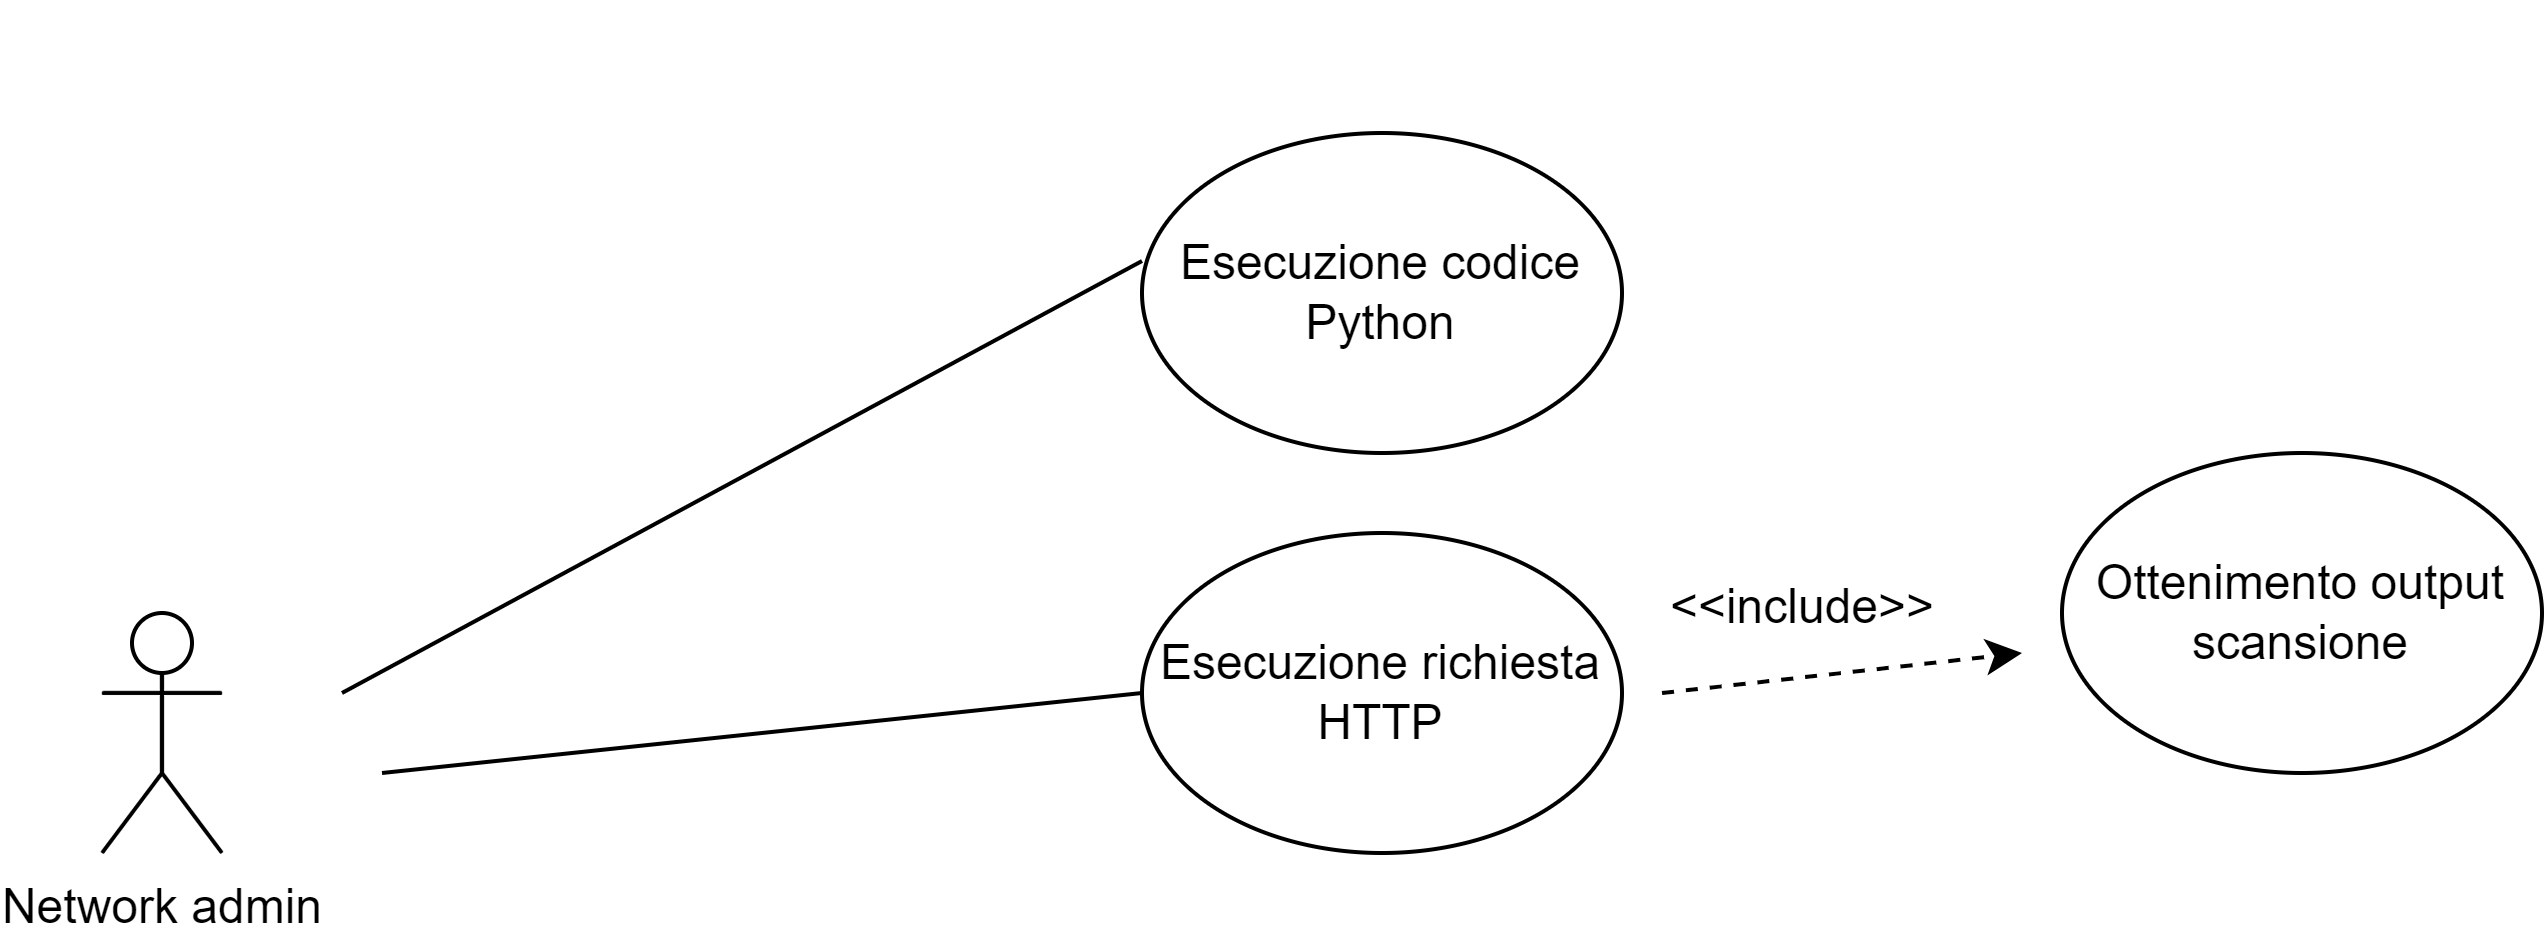
\includegraphics[width=0.7\textwidth] {Tesi magistrale/capitoli/images/use case 1.png}
\centering
\caption{Use case modulo scansione.}
\end{figure}

\subsection{Use case modulo VPN}
Come si evince dall’immagine sottostante, il modulo VPN viene anch’esso gestito da una figura preposta a tale lavoro; mentre i vari client che desiderano connettersi al \emph{server VPN} hanno la possibilità di usufruire del servizio finale cioè entrare a far parte della rete LAN del dispositivo o navigare in modo sicuro.

\begin{figure}[h] 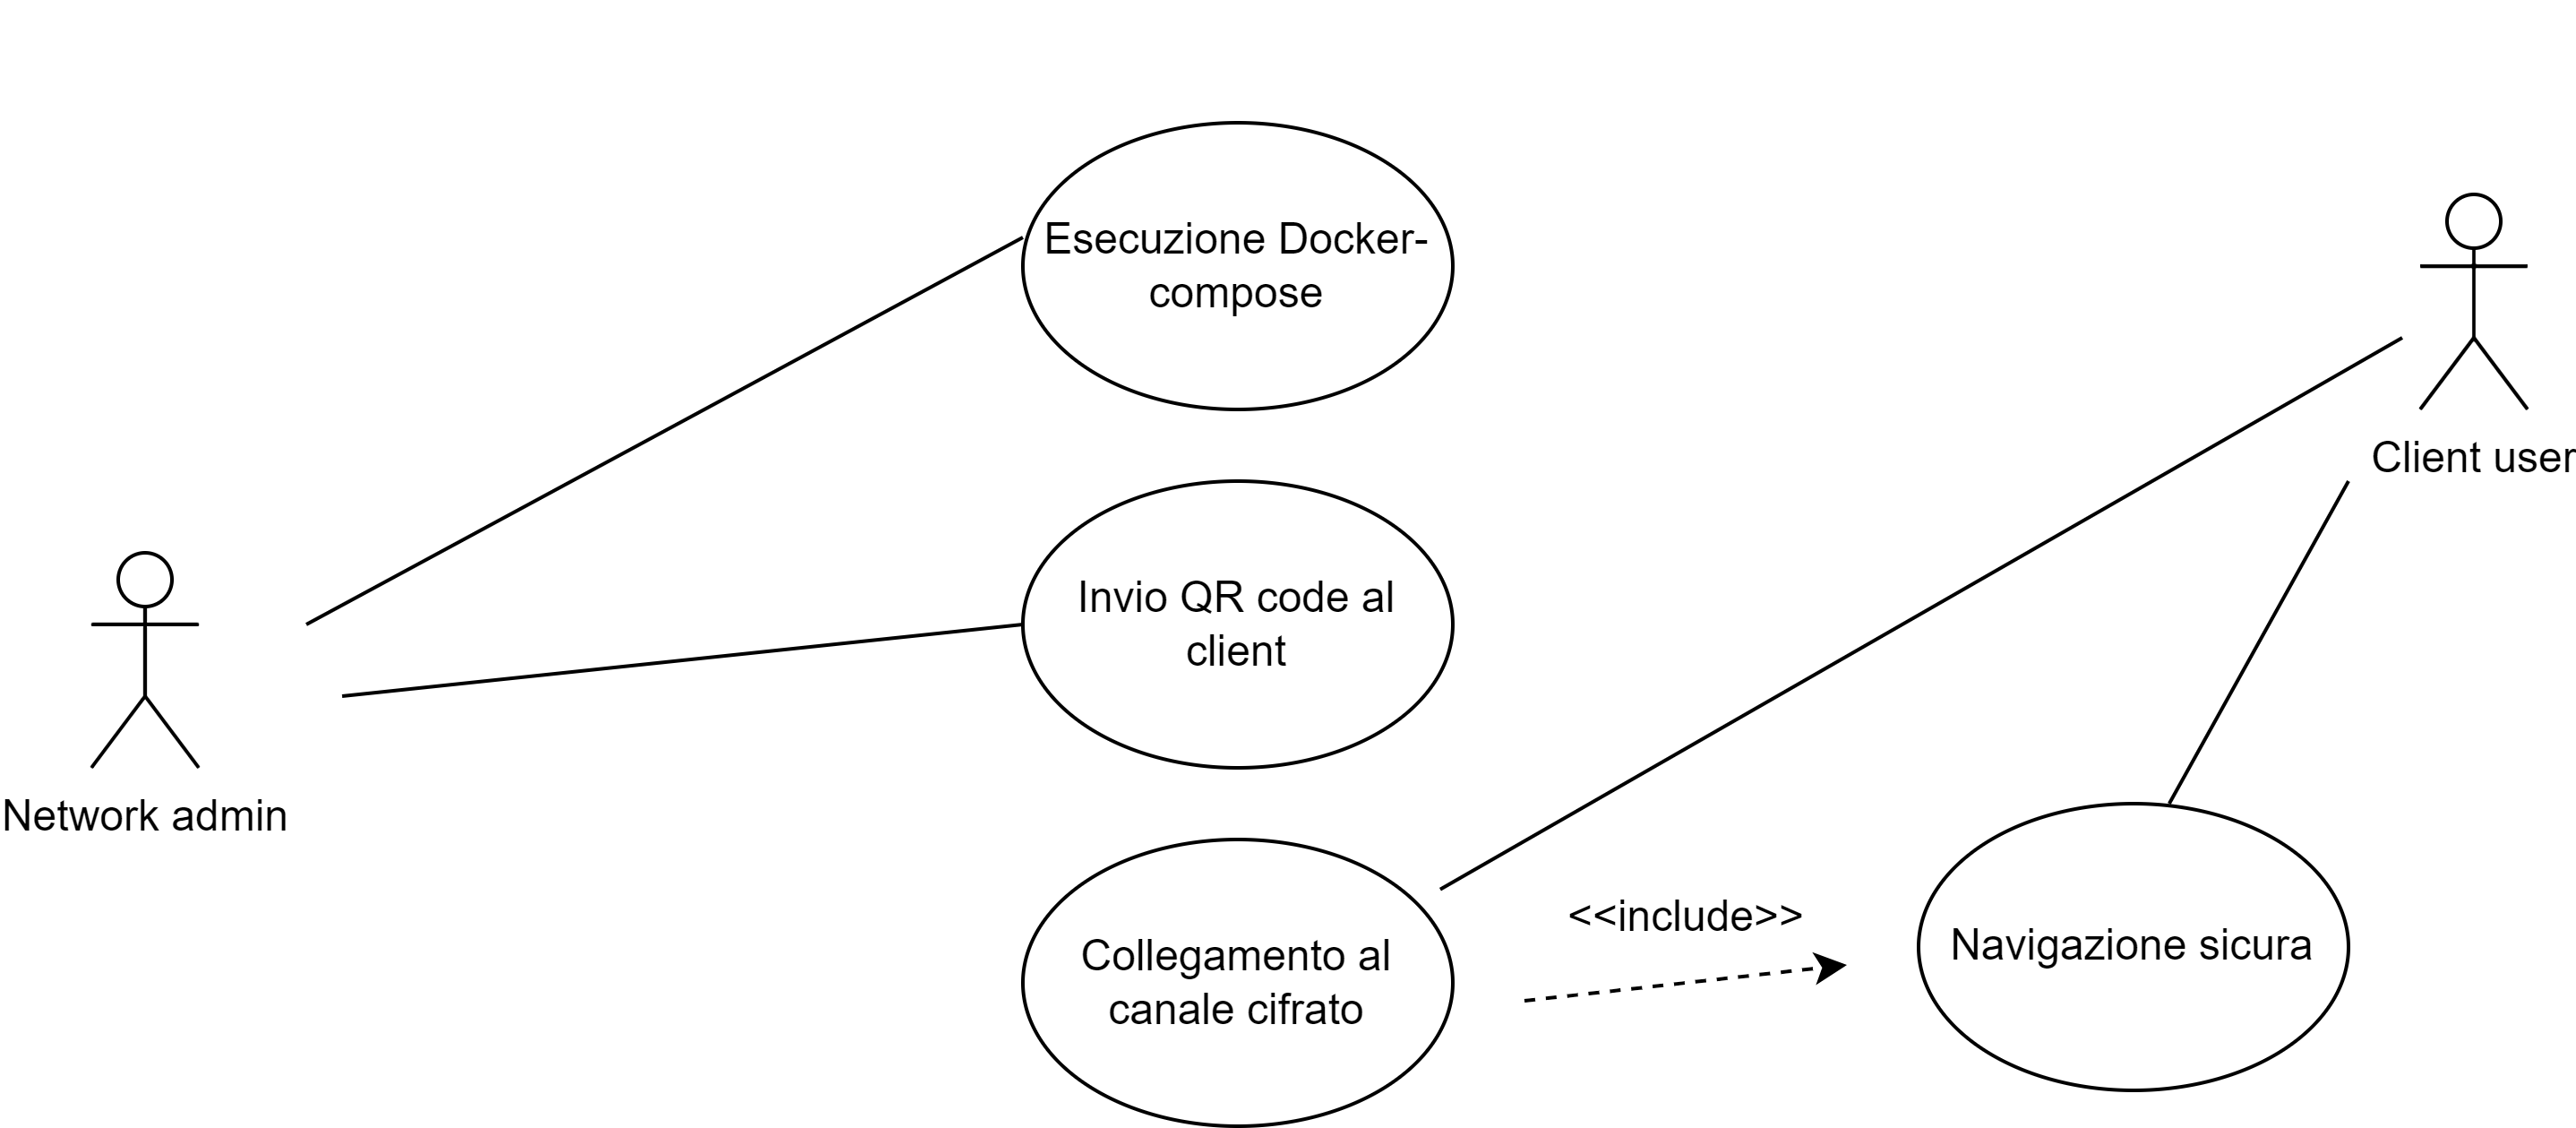
\includegraphics[width=0.7\textwidth] {Tesi magistrale/capitoli/images/use case 2.png}
\centering
\caption{Use case modulo VPN.}
\end{figure}

\section{Conclusioni}
I requisiti raccolti in questa fase saranno successivamente impiegati per la progettazione e l'implementazione del sistema proposto.

\include{capitoli/Progettazione}
\chapter{Realizzazione del sistema proposto} %\label{1cap:spinta_laterale}
% [titolo ridotto se non ci dovesse stare] {titolo completo}
%

\begin{citazione}
In questo capitolo, le idee e i concetti, definiti precedentemente, saranno realizzati sotto forma di codice funzionante. Attraverso l’implementazione, il sistema prenderà forma, diventando un prodotto software pronto per essere impiegato nella risoluzione dei compiti preposti.
\end{citazione}
\newpage

Come ampiamente esplicitato nei capitoli precedenti, l'obiettivo principale del lavoro svolto è quello di poter analizzare il comportamento di determinati flussi di dati con particolari requisiti di \emph{QoS} in relazione all'utilizzo di diversi protocolli VPN. Vediamo ora nel dettaglio come è stato svolto questo compito.
\subsection{Utilizzo dei protocolli VPN}
Per quanto riguarda l'utilizzo dei protocolli VPN, come è stato presentato nei capitoli precedenti, è stato scelto di utilizzare tre diversi protocolli affinché siano ben chiare le performance ottenibili tramite il loro impiego. I flussi di test precedentemente definiti sono stati scambiati tra client e server i quali sono stati messi in comunicazione tramite l'attivazione di un singolo protocollo VPN per volta in modo da stabilire un canale di comunicazione \emph{cifrato} tra loro. 
Tutti i test eseguiti sono stati portati avanti utilizzando i  protocolli VPN installati \emph{localmente} al sistema realizzato così da evitare l'utilizzo di \emph{container} che avrebbero potuto compromettere i risultati finali dei test.

\section{Sviluppo e integrazione  modulo scansione}
Passiamo ora all'implementazione vera e propria del modulo adibito all'esecuzione delle scansioni dei dispositivi presenti in rete. Come è stato accennato nel capitolo precedente, il presente modulo è stato realizzato impiegando \emph{Python} come linguaggio di programmazione proprio perché offre la possibilità di poter integrare numerose librerie utili allo sviluppo del codice tra cui \emph{Nmap}, \emph{Flask} e \emph{Celery}. Nella figura 5.1 è possibile notare la struttura del progetto realizzato ed i file che lo compongono.
\begin{figure}[h] 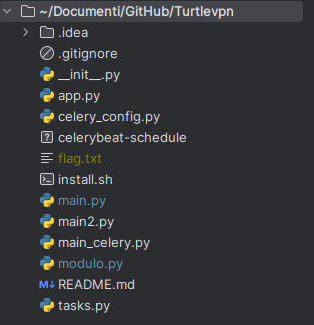
\includegraphics[width=0.5\textwidth] {Tesi magistrale/capitoli/images/file progetto.png}
\centering
\caption{File del progetto.}
\end{figure}

Passiamo ora ad analizzare i principali file che implementano le funzionalità del sistema in questione.

\subsection{modulo.py}
Questo file contiene tutte le scansioni implementate tramite l'utilizzo della libreria \emph{Nmap}. ogni scansione genera un file di output \emph{testuale}, così da poter consultare i risultati anche in un secondo momento dopo la scansione; in particolare sono state implementate diverse scansioni affinché sia possibile cogliere diversi aspetti riguardanti gli host in rete:
\begin{itemize}
    \item \emph{scans (indirizzo)}: elenca i diversi host presenti in rete;
    \item \emph{scans\_time (indirizzo, timer)}: scansione periodica della rete;
    \item \emph{scan\_port (indirizzo, porte)}: scansione di determinate porte;
    \item \emph{scan\_service (indirizzo)}: scansione dei servizi presenti su un indirizzo;
    \item \emph{scan\_os (indirizzo)}: scansione del sistema operativo degli host;
    \item \emph{scan\_vuln (indirizzo)}: scansione delle vulnerabilità degli host.
\end{itemize}

Nella figura 5.2 è riportato un esempio di scansione, in particolare è l'implementazione della scansione \emph{scan\_port}. Per completezza è possibile consultare le altre scansioni all'interno del progetto \emph{GitHub} \cite{pro}.
\begin{figure}[h] 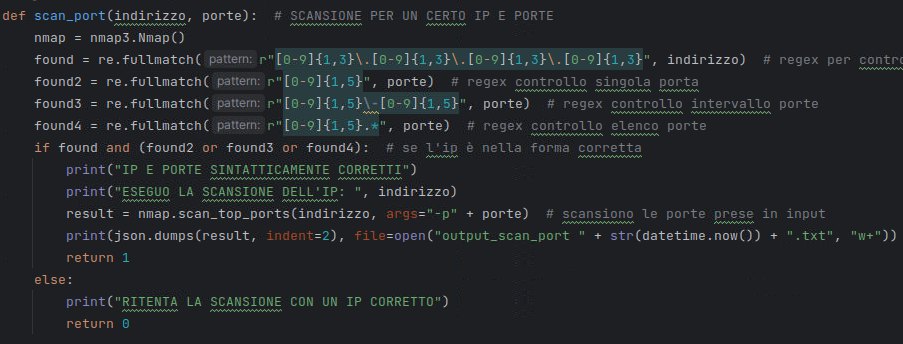
\includegraphics[width=1\textwidth] {Tesi magistrale/capitoli/images/scan.png}
\centering
\caption{Esempio scansione: scan\_port.}
\end{figure}

\subsection{tasks.py}
In questo file sono stati definiti i diversi \emph{task} eseguibili tramite l’impiego di \emph{Celery}, uno scheduler Open Source che permette di programmare l’esecuzione dei task ed anche di eseguirli in modo \emph{asincrono} così da non bloccare l’esecuzione e l’interattività di una pagina web. Nella figura seguente è riportata la definizione di un task per Celery; ovviamente tutti gli altri task sono presenti nel progetto \emph{GitHub} \cite{pro}.
\begin{figure}[h] 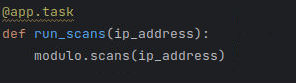
\includegraphics[width=0.5\textwidth] {Tesi magistrale/capitoli/images/task.png}
\centering
\caption{Task per Celery.}
\end{figure}

\subsection{app.py}
In questo file sono state definite le varie \emph{richieste HTTP} in modo da poter utilizzare i task, definiti precedentemente, anche richiamandoli da una possibile pagina web. Le diverse richieste sono state realizzate tramite l’utilizzo di \emph{Flask}, un particolare framework per lo sviluppo web backend in Python.

\begin{figure}[h] 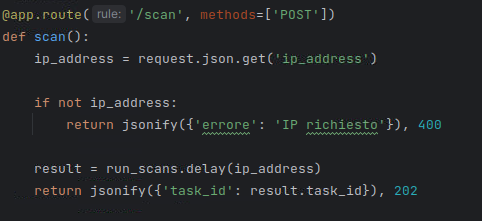
\includegraphics[width=0.6\textwidth] {Tesi magistrale/capitoli/images/app.png}
\centering
\caption{Task per Flask.}
\end{figure}

\section{Sviluppo e integrazione modulo VPN}
In questa sezione è stato sviluppato il modulo inerente all'impiego del protocollo \emph{WireGuard} versione \emph{standard} per fornire agli utenti la possibilità di accedere alle risorse presenti nella rete a cui è connesso il sistema \emph{TurtleVPN} oltre che a fornire la possibilità di poter navigare in rete in modo sicuro.

\subsection{WireGuard e Docker}
A tale scopo è stato utilizzato il gestore di container \emph{Docker} il quale permette di poter gestire in modo agevole i diversi container in cui sono stati istanziati gli applicativi di interesse. In questo caso la versione di Docker utilizzata è la \emph{Compose} \cite{compose} che a differenza della versione standard permette di poter gestire più container allo stesso tempo, di conseguenza offre la possibilità di poter estendere o implementare nuove funzionalità legale all'utilizzo del protocollo WireGuard. Nella figura 5.5 è possibile osservare la configurazione del file \emph{docker-compose.yaml} il quale ha il compito di istanziare i servizi definiti all'interno di esso in base alla configurazione scelta.
\begin{figure}[h] 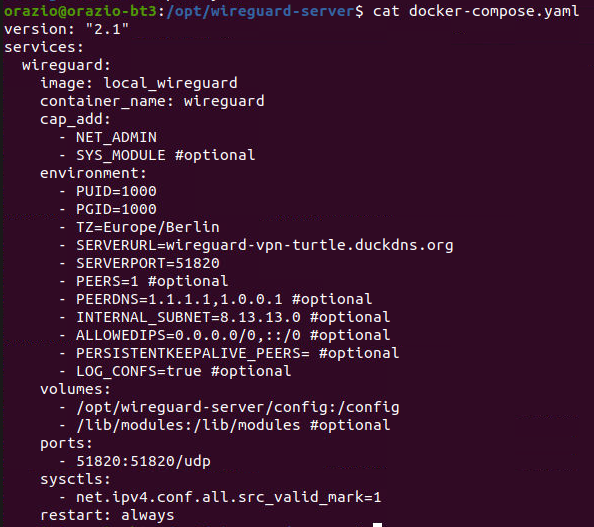
\includegraphics[width=0.6\textwidth] {Tesi magistrale/capitoli/images/wire.png}
\centering
\caption{File docker-compose.yaml.}
\end{figure}

\subsubsection{docker-compose.yaml}
Alcuni dettagli presenti nel file di configurazione:
\begin{itemize}
    \item L'immagine di WireGuard è presente localmente al sistema;
    \item L'indirizzo \emph{reale} del server è stato impostato in modo da fare sempre riferimento all'indirizzo \emph{pubblico} della rete a cui è connesso TurtleVPN in modo che i client possano sempre navigare utilizzando quell'indirizzo. Per raggiungere questo obiettivo è stato impiegato il servizio \emph{Duck DNS} \cite{duck} il quale permette di assegnare ad una stringa l'indirizzo di rete pubblico e di gestire in maniera automatica l'indirizzo di rete fornito dal \emph{provider} anche nel caso in cui cambi dopo un certo lasso di tempo;
    \item La connessione al server WireGuard avviene tramite la porta \emph{51820 UDP};
    \item \emph{8.13.13.0/24} rappresenta la \emph{subnet} assegnata ai dispositivi connessi a TurtleVPN utilizzando un canale sicuro instaurato tramite WireGuard;
\end{itemize}

\subsection{WireGuard client}
Relativamente ai dispositivi client che intendono connettersi al server VPN è necessario che essi eseguano l'\emph{import} del file di configurazione che è stato generato dall'applicativo server WireGuard in esecuzione nel sistema; per i dispositivi mobili è possibile anche effettuare la scansione del \emph{QR-Code} così da poter eseguire l'importazione della configurazione in modo agevole all'interno dell'applicazione client. Nella figura 5.6 è mostrata la configurazione per un client.
\begin{figure}[h] 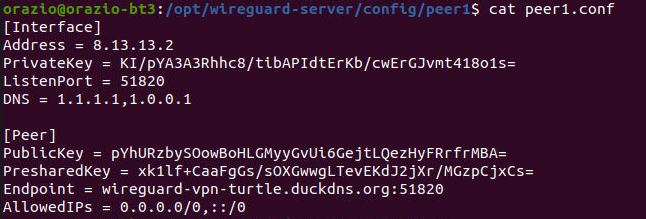
\includegraphics[width=0.7\textwidth] {Tesi magistrale/capitoli/images/confcli.png}
\centering
\caption{Configurazione WireGuard client.}
\end{figure}
\chapter{Testing e valutazione delle prestazioni del sistema} 

\begin{citazione}
In questa sezione, il sistema sarà messo alla prova, misurando le sue prestazioni in termini di velocità, efficienza e affidabilità. Questo permetterà di individuare eventuali aree di miglioramento e di ottimizzare il sistema per garantire la migliore esperienza possibile agli utenti finali.
\end{citazione}
\newpage

\section{Progettazione dei test}
Come è stato spiegato nel capitolo \emph{Progettazione}, alla base di ogni esperimento è stato definito un preciso \emph{flusso di dati} avente dei requisiti di \emph{QoS}. Sono stati presi in considerazione i flussi che al giorno d'oggi sono maggiormente utilizzati nell'ambito delle comunicazioni e di fornitura di determinati servizi web based. Sotto sono riportati i flussi che sono stati presi in considerazione per gli esperimenti da eseguire; ogni flusso ha il compito di simulare uno specifico servizio nel modo più fedele possibile: 
\newline
\begin{itemize}
    \item Flusso UDP per misurare il \emph{throughput} massimo;
    \item Flusso TCP per misurare il \emph{throughput} massimo;
    \item Flusso UDP per simulare il protocollo \emph{VoIP};
    \item Flusso per simulare uno \emph{streaming video};
    \item Flusso per simulare un \emph{trasferimento massivo}.
\end{itemize} 

\section{Implementazione dei flussi con iPerf}
Nel paragrafo precedente sono stati progettati i diversi flussi di dati da utilizzare per i vari test da eseguire; per la realizzazione vera e propria si è scelto di utilizzare \emph{iPerf} il quale permette di poter simulare un flusso di dati in maniera molto precisa tramite l'utilizzo di numerosi \emph{flag} e di poter gestire lo scambio di dati tra un \emph{server} ed un \emph{client} i quali eseguono entrambi il tool. Sotto è riportata la definizione esatta dei comandi per simulare i flussi:
\begin{itemize}
    \item \fcolorbox{black}{red!5}{.\textbackslash iperf3 -c 10.66.66.1 -p 2020 -u -b 0 -n 512M --get-server-output;} \newline
    Questo comando simula l'invio di 512 MB tramite il protocollo di rete UDP, utilizzando tutta la banda disponibile.
    \item \fcolorbox{black}{red!5}{.\textbackslash iperf3 -c 10.66.66.1 -p 2020 -P 10 -b 0 -w 100k --get-server-output;} \newline
    Questo flusso simula l'invio di pacchetti TCP utilizzando dieci connessioni parallele verso il server ed la massima banda disponibile.
    \item \fcolorbox{black}{red!5}{.\textbackslash iperf3 -c 10.66.66.1 -u -p 2020 -S 0x28 -l 78 -b 100K --get-server-output;} \newline
    Questo flusso simula l'invio di pacchetti UDP appartenenti ad un flusso di dati di tipo VoIP.
    \item \fcolorbox{black}{red!5}{.\textbackslash iperf3 -c 10.66.66.1 -p 2020 -S 32 -M 1460B --get-server-output;} \newline
    Questo flusso simula l'invio di pacchetti TCP appartenenti ad un flusso di streaming video.
    \item .\textbackslash \fcolorbox{black}{red!5}{.\textbackslash iperf3 -c 10.66.66.1 -p 2020 -S 10 -M 1460B -b 0 --get-server-output;} \newline
    Questo flusso simula l'invio di pacchetti TCP appartenenti ad un flusso bulk data cioè di trasferimento di massa.
\end{itemize}
\subsubsection{Dettagli sui flag utilizzati}
Al fine di comprendere a pieno come sono stati simulati i diversi flussi di dati scambiati negli esperimenti tra client e server, è importante capire il significato dei \emph{flag} utilizzati:
\begin{itemize}
    \item \emph{-c}: Indirizzo dell'host che esegue iPerf server;
    \item \emph{-p}: Porta in ascolto di iPerf server;
    \item \emph{-u}: Flusso di tipo UDP;
    \item \emph{-b}: Banda disponibile per il trasferimento. 0 indica che la banda è massima;
    \item \emph{-n}: Quantità di byte da inviare durante il test;
    \item \emph{-P}: Numero di connessioni parallele del client;
    \item \emph{-S}: Assegna ai pacchetti una determinata priorità per simulare i pacchetti di un preciso protocollo applicativo;
    \item \emph{-M}: Grandezza massima del singolo pacchetto TCP;
    \item \emph{--get-server-output}: L'output del test viene visualizzato anche sul client.
\end{itemize}

\section{Definizione metriche di valutazione}
Arrivati a questo punto del lavoro è molto importante capire sulla base di quali \emph{parametri} effettuare la valutazione del sistema realizzato in modo da poter stabilire con certezza l'efficacia di esso. A tal proposito, è stato scelto di rendere le valutazioni degli esperimenti del tutto indipendenti tra loro; in particolare i diversi esperimenti sono stati valutati in base ai valori assunti principalmente dai due seguenti parametri:

\begin{itemize}
    \item \emph{Bitrate}: Indica la quantità di informazioni che sono state trasferite in un'unica unità di tempo;
    \item \emph{Trasferimento}: Indica la quantità di informazioni trasferite durante l'esecuzione dell'intero test.
\end{itemize}

I parametri sopracitati sono di fondamentale importanza affinché si possa stabilire se le \emph{condizioni di rete}, derivanti anche dall'utilizzo o meno di uno dei protocolli VPN, siano adatte per consentire il corretto impiego dei flussi stabiliti.

\section{Esecuzione degli esperimenti e analisi dei risultati}
Il passo successivo è quello di proseguire con l'esecuzione degli esperimenti prefissati in modo da poter raccogliere i dati di output e poterli utilizzare per la generazione di \emph{grafici} da utilizzare come strumento di ausilio all'analisi degli output stessi. Al fine di evitare ripetizioni superflue è stato evitato di trattare ogni singola esecuzione di ogni test per cui nel paragrafo successivo è riportato un singolo campione di esecuzione che rispecchia la struttura di tutte le altre indipendentemente dal protocollo VPN utilizzato. I dati di output di tutte le esecuzioni dei test sono presenti nel progetto \emph{GitHub} \cite{pro}.

\subsection{Esempio di esecuzione test}
Nel seguente sottoparagrafo è riportato un esempio di una singola esecuzione del test \emph{numero 1} tra il sistema TurtleVPN ed un client, avente sistema operativo \emph{Windows 11}, il quale invia il flusso di dati in modo da poter ricevere i risultati di output. Nella figura 6.1 è rappresentata l'esecuzione del comando per fare in modo che TurtleVPN possa ricevere il flusso di dati prestabilito che sarà inviato dal client, come in figura 6.2, il quale riceverà anche l'output dell'esecuzione. Ogni esperimento è stato eseguito allo stesso modo indipendentemente dal protocollo VPN impiegato. Da come si nota dalla figura 6.2, l'output del test è suddiviso in intervalli i quali sono numericamente differenti in base al tipo di flusso simulato.

\begin{figure}[h] 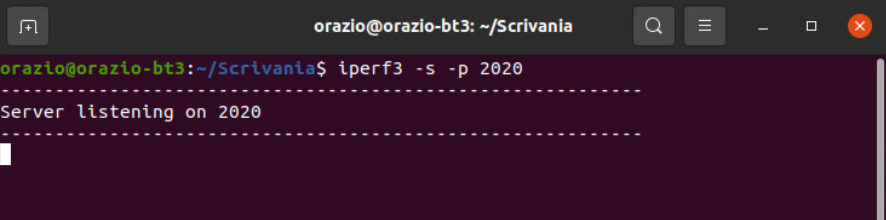
\includegraphics[width=0.6\textwidth] {Tesi magistrale/capitoli/images/iPerf server.png}
\centering
\caption{Comando iPerf server.}
\end{figure}

\begin{figure}[h] 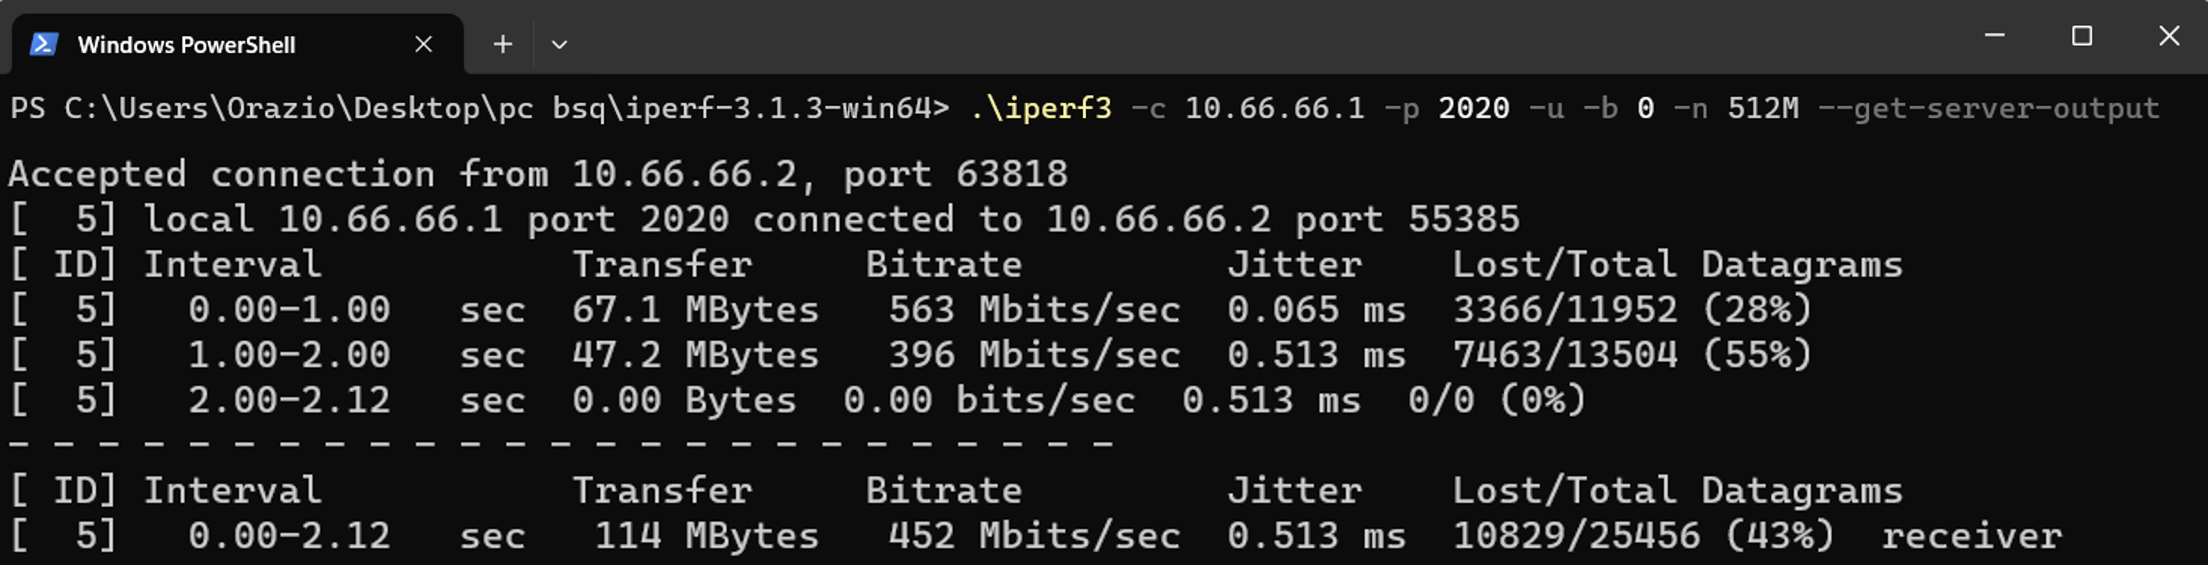
\includegraphics[width=0.7\textwidth] {Tesi magistrale/capitoli/images/iPerf client.png}
\centering
\caption{Comando iPerf client.}
\end{figure}

\newpage

Sulla base degli output ottenuti dalle varie esecuzioni di ogni test, saranno estrapolate le considerazioni sui protocolli VPN, grazie anche ai grafici generati a partire proprio dai dati di output dei test.

\section{Analisi dei risultati}
Analizziamo ora i risultati ottenuti dai test; in particolare i grafici riguardano i parametri \emph{bitrate} e \emph{transfer} ottenuti in output da ogni esecuzione. Per ogni esperimento sono quindi stati creati \emph{due} grafici per ognuna delle \emph{dieci} esecuzioni del test in modo da avere una visione chiara dell'andamento dell'esperimento, inoltre per ogni esperimento sono stati generati anche due grafici ad istogramma rappresentanti \emph{bitarte} e \emph{transfer} medio. Visto che ogni esperimento è stato eseguito con diversi protocolli VPN, si eviterà di mostrare tutti i grafici affinché si possa cogliere il senso di ogni esperimento; il set di grafici completo è presente nel progetto \emph{GitHub} \cite{pro}.

\newpage
\subsection{Primo esperimento}
L'esperimento in questione riguarda l'invio di 512 MB tramite l'utilizzo del protocollo UDP, sfruttando tutta la banda di rete disponibile.

\subsubsection{Grafici esperimento senza VPN}

\begin{figure}[h] 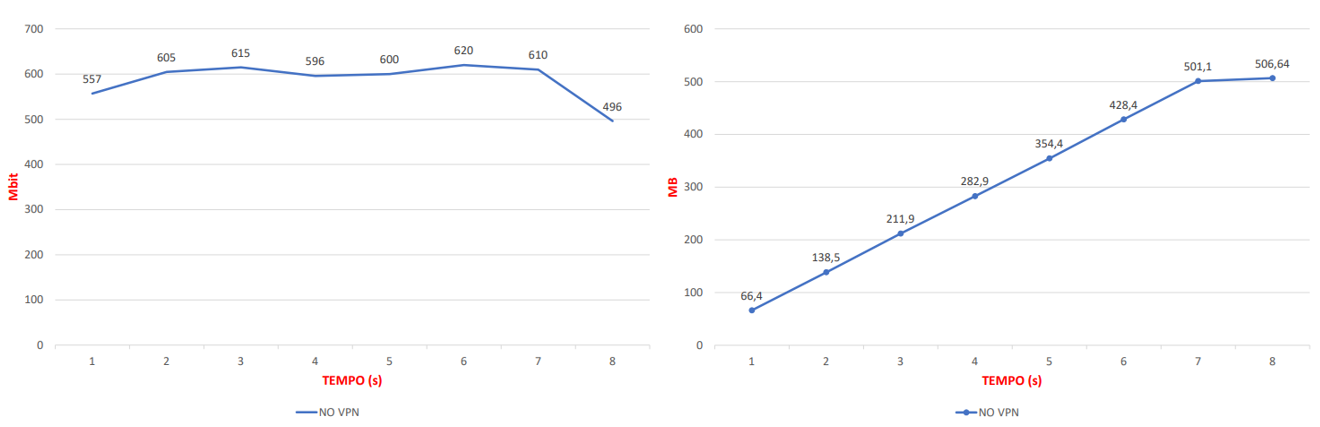
\includegraphics[width=0.9\textwidth] {Tesi magistrale/capitoli/images/1.png}
\centering
\caption{Grafici 1° esecuzione.}
\end{figure}

\begin{figure}[h] 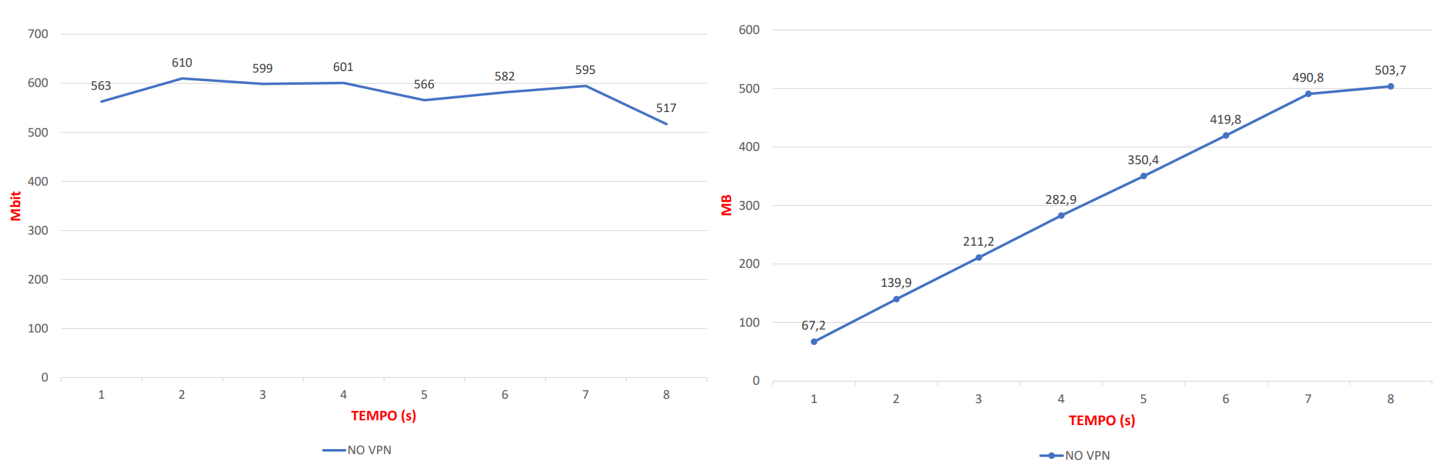
\includegraphics[width=0.9\textwidth] {Tesi magistrale/capitoli/images/2.png}
\centering
\caption{Grafici 5° esecuzione.}
\end{figure}

\begin{figure}[h] 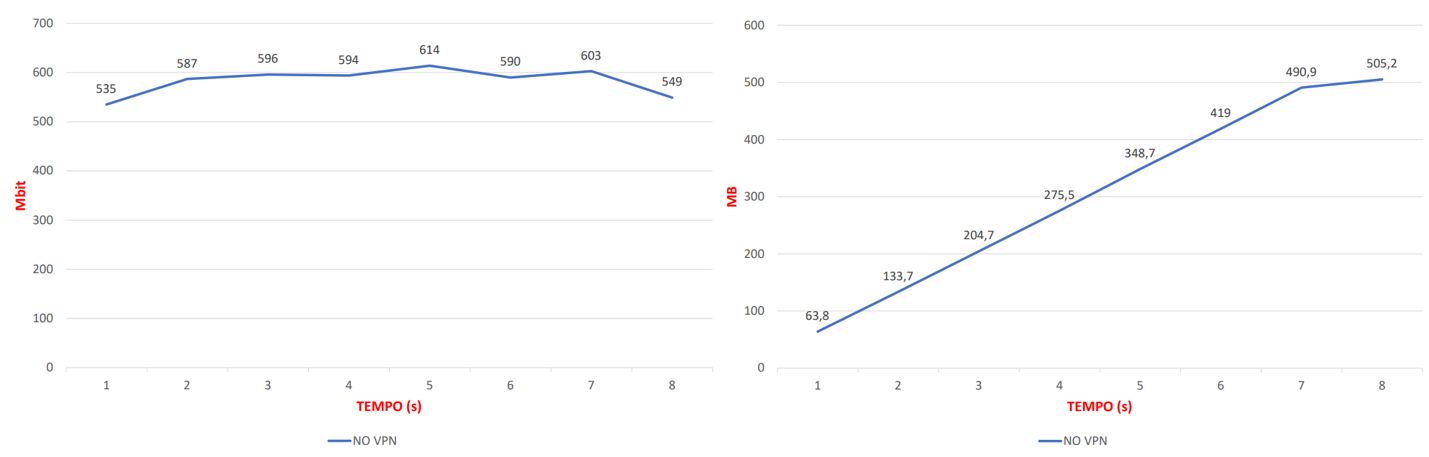
\includegraphics[width=0.9\textwidth] {Tesi magistrale/capitoli/images/3.png}
\centering
\caption{Grafici 10° esecuzione.}
\end{figure}

\newpage
\subsubsection{Grafici esperimento con WireGuard standard}

\begin{figure}[h] 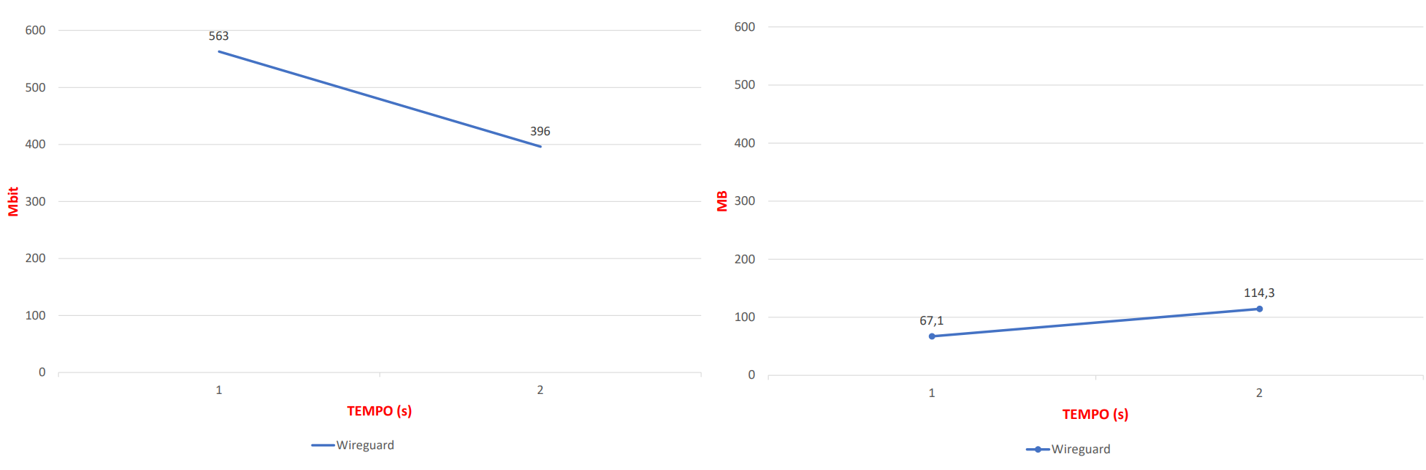
\includegraphics[width=0.9\textwidth] {Tesi magistrale/capitoli/images/4.png}
\centering
\caption{Grafici 1° esecuzione.}
\end{figure}

\begin{figure}[h] 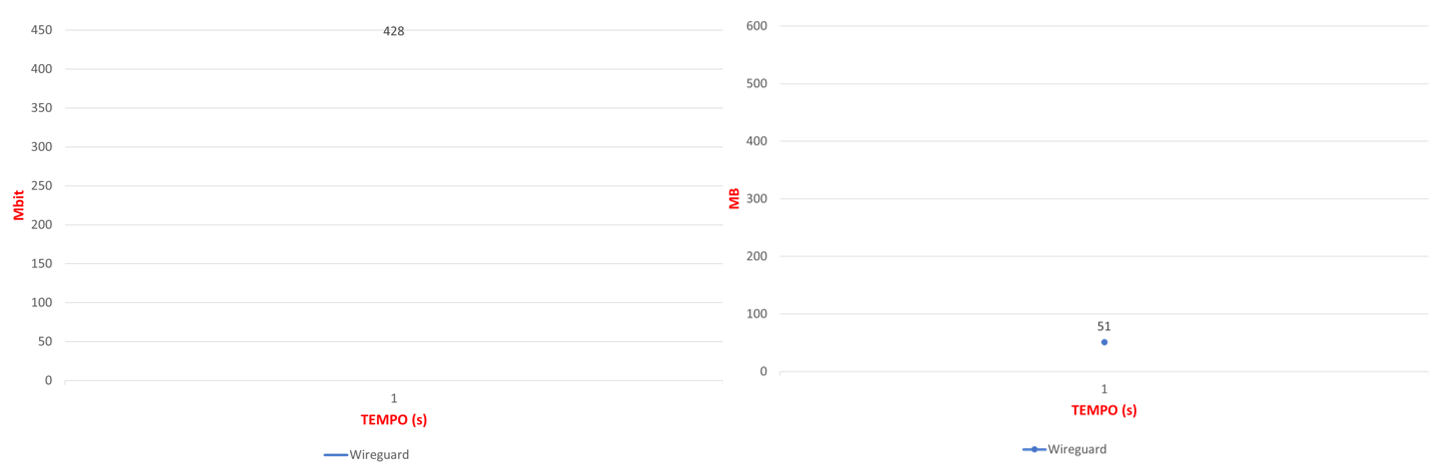
\includegraphics[width=0.9\textwidth] {Tesi magistrale/capitoli/images/5.png}
\centering
\caption{Grafici 5° esecuzione.}
\end{figure}

\begin{figure}[h] 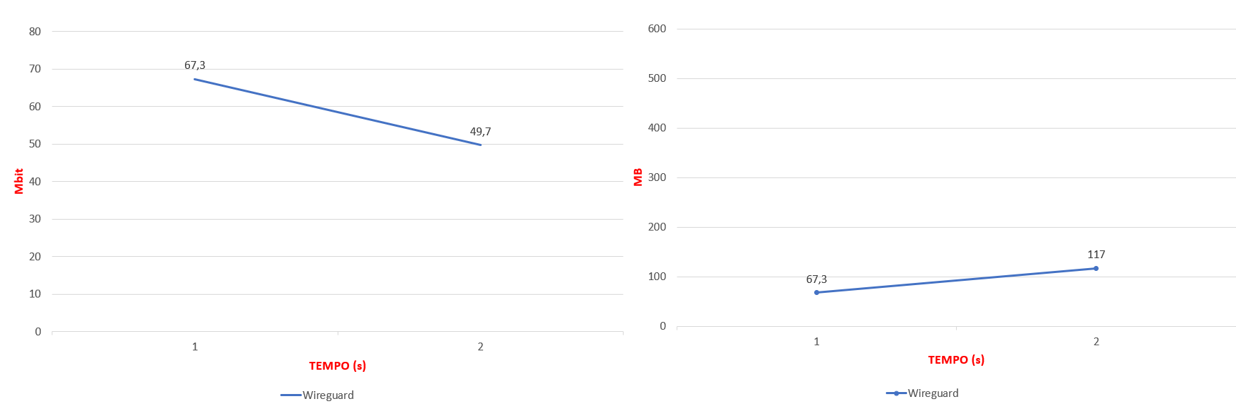
\includegraphics[width=0.9\textwidth] {Tesi magistrale/capitoli/images/6.png}
\centering
\caption{Grafici 10° esecuzione.}
\end{figure}

\newpage
\subsubsection{Grafici esperimento con WireGuard PQ}

\begin{figure}[h] 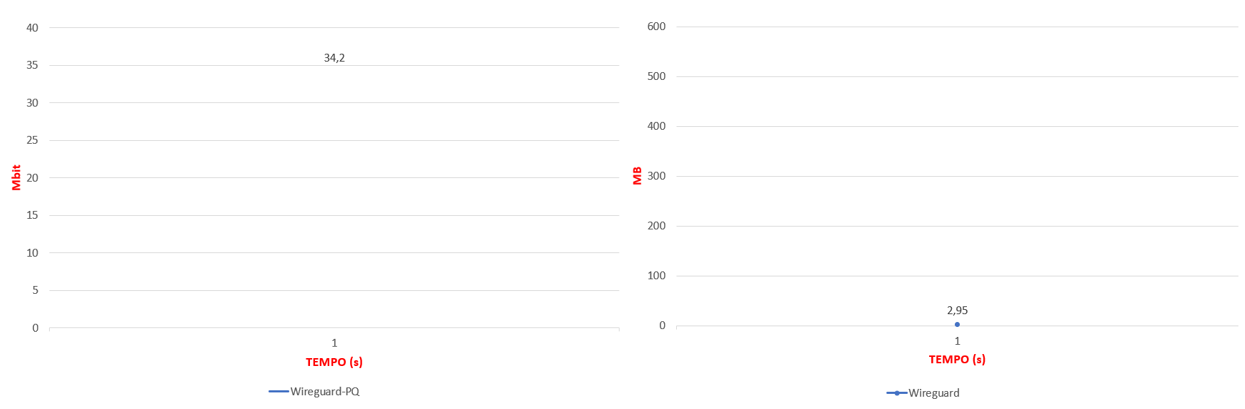
\includegraphics[width=0.9\textwidth] {Tesi magistrale/capitoli/images/7.png}
\centering
\caption{Grafici 1° esecuzione.}
\end{figure}

\begin{figure}[h] 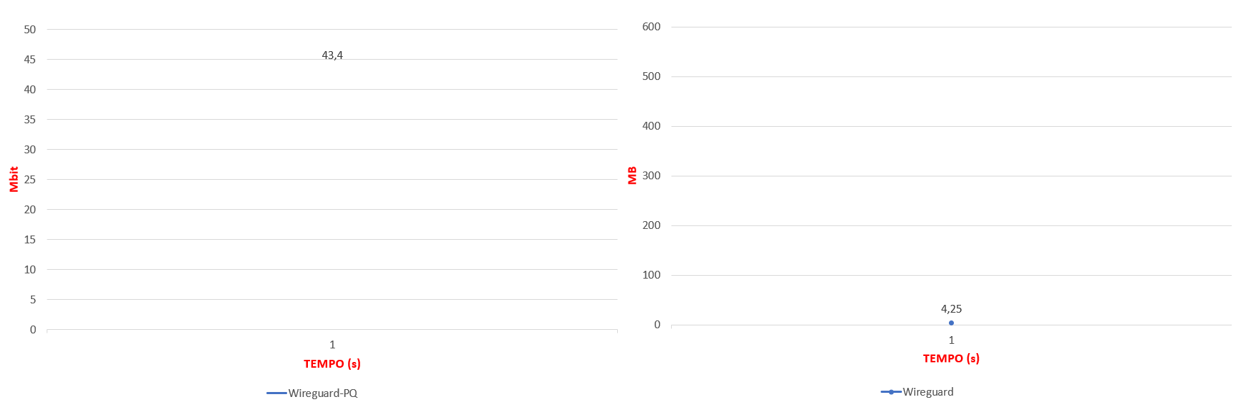
\includegraphics[width=0.9\textwidth] {Tesi magistrale/capitoli/images/8.png}
\centering
\caption{Grafici 5° esecuzione.}
\end{figure}

\begin{figure}[h] 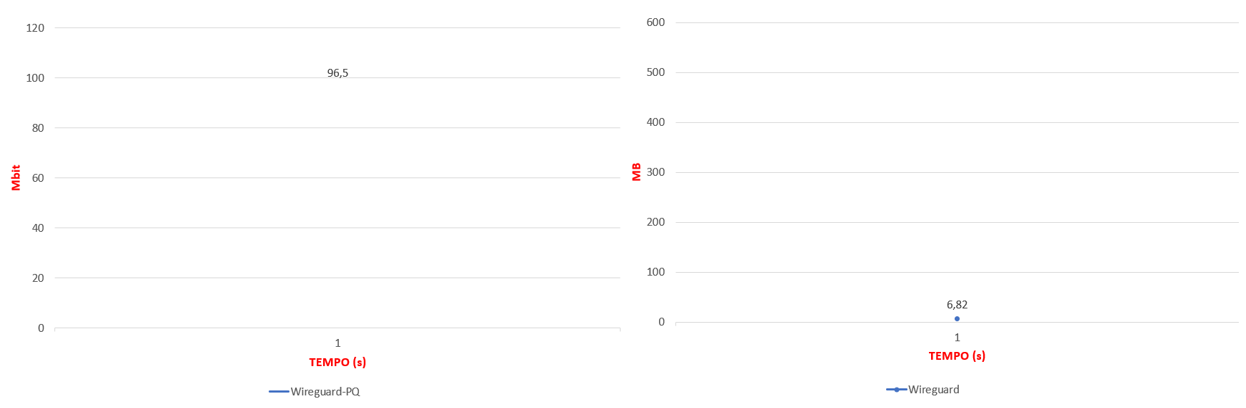
\includegraphics[width=0.9\textwidth] {Tesi magistrale/capitoli/images/9.png}
\centering
\caption{Grafici 10° esecuzione.}
\end{figure}

\newpage
\subsubsection{Grafici esperimento con OpenVPN}

\begin{figure}[h] 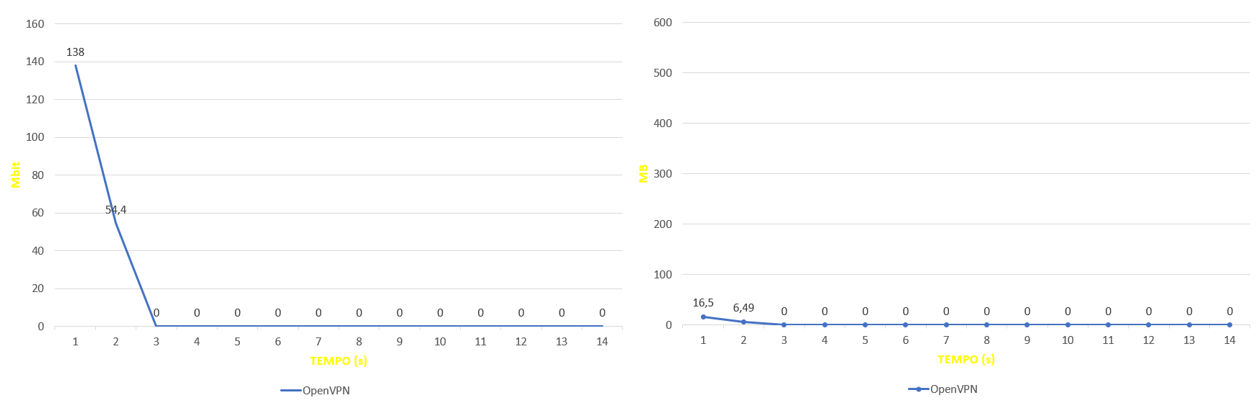
\includegraphics[width=0.9\textwidth] {Tesi magistrale/capitoli/images/10.png}
\centering
\caption{Grafici 1° esecuzione.}
\end{figure}

\begin{figure}[h] 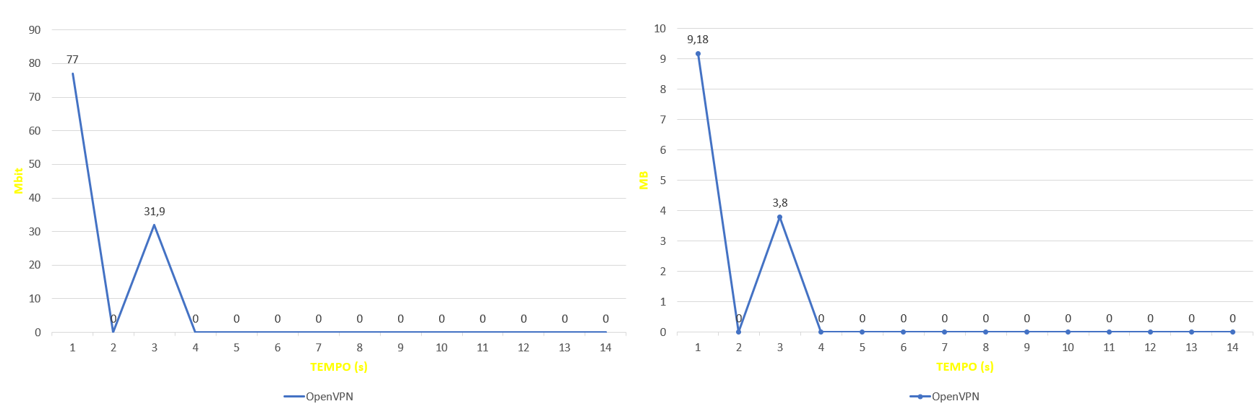
\includegraphics[width=0.9\textwidth] {Tesi magistrale/capitoli/images/11.png}
\centering
\caption{Grafici 5° esecuzione.}
\end{figure}

\begin{figure}[h] 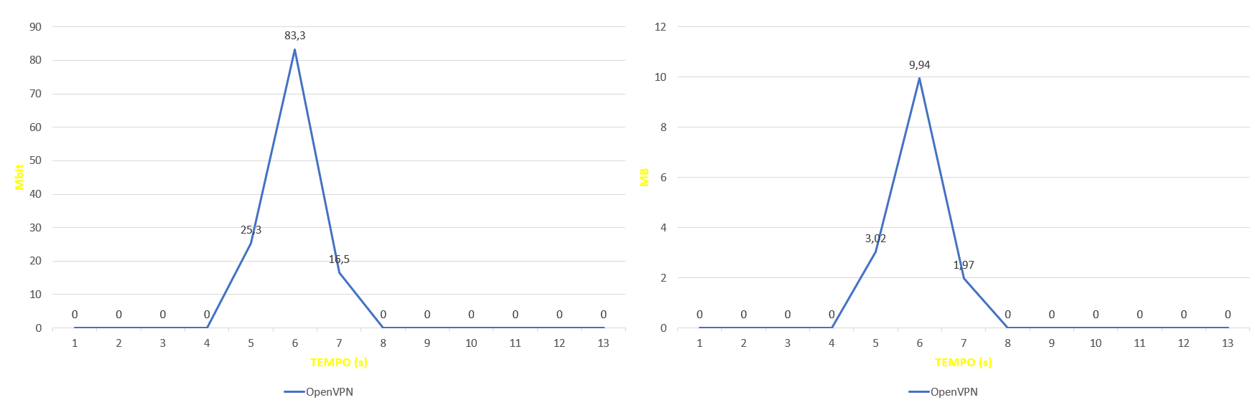
\includegraphics[width=0.9\textwidth] {Tesi magistrale/capitoli/images/12.png}
\centering
\caption{Grafici 10° esecuzione.}
\end{figure}

\newpage
\subsubsection{Grafici riassuntivi}

\begin{figure}[h] 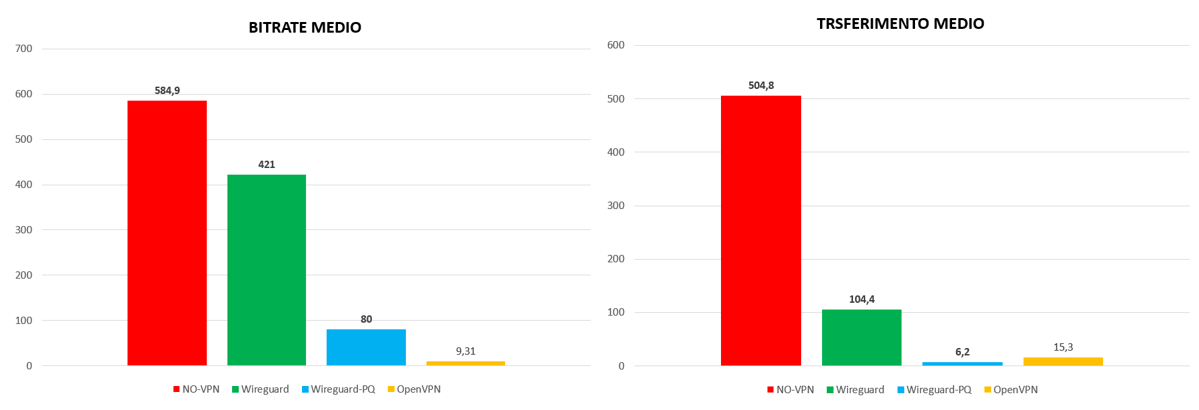
\includegraphics[width=1\textwidth] {Tesi magistrale/capitoli/images/13.png}
\centering
\caption{Grafici riassuntivi.}
\end{figure}

\subsubsection{Esito primo esperimento}
Dai grafici si può notare che ovviamente l'esperimento restituisce i risultati migliori quando nessun protocollo VPN è attivo; mentre tra le diverse VPN testate quella che si comporta meglio è sicuramente \emph{WireGuard standard} il quale offre prestazioni migliori almeno in questo esperimento. 

\newpage
\subsection{Secondo esperimento}
Il secondo esperimento riguarda l'invio di numerosi pacchetti tramite l'utilizzo del protocollo TCP e di dieci connessioni parallele verso il server iPerf in modo da poter stabilire principalmente il throughput massimo raggiungibile.
\subsubsection{Grafici esperimento senza VPN}

\begin{figure}[h] 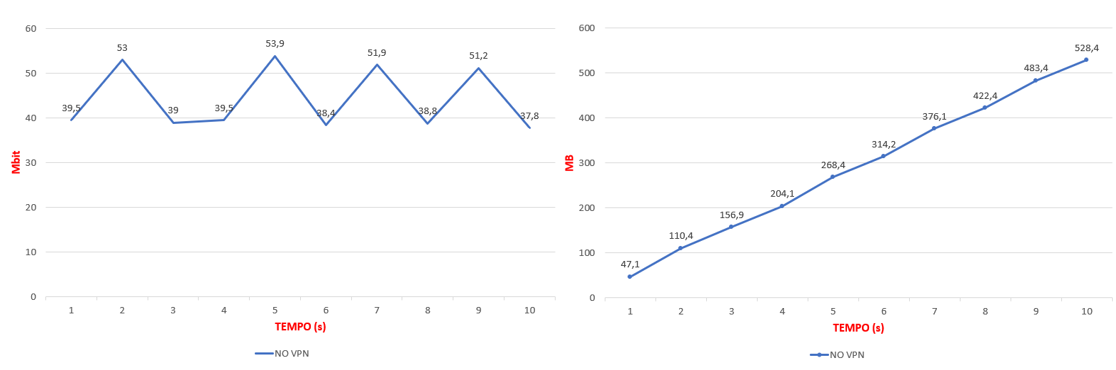
\includegraphics[width=0.9\textwidth] {Tesi magistrale/capitoli/images/14.png}
\centering
\caption{Grafici 1° esecuzione.}
\end{figure}

\begin{figure}[h] 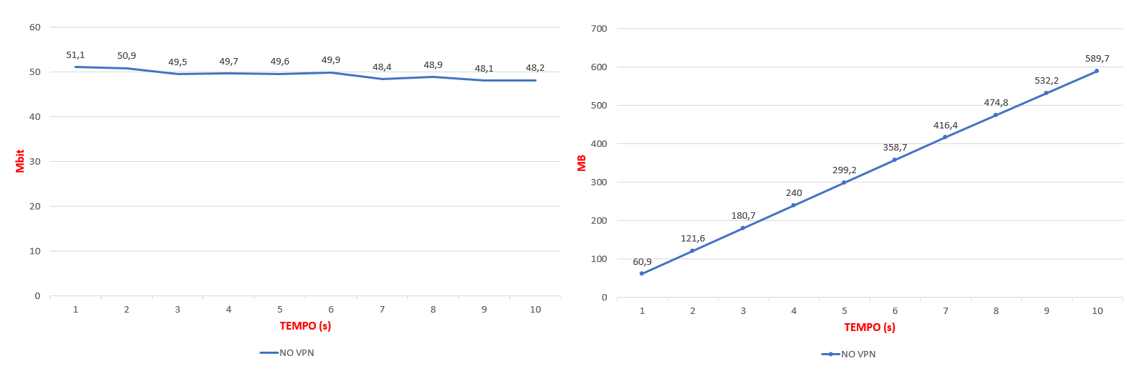
\includegraphics[width=0.9\textwidth] {Tesi magistrale/capitoli/images/15.png}
\centering
\caption{Grafici 5° esecuzione.}
\end{figure}

\begin{figure}[h] 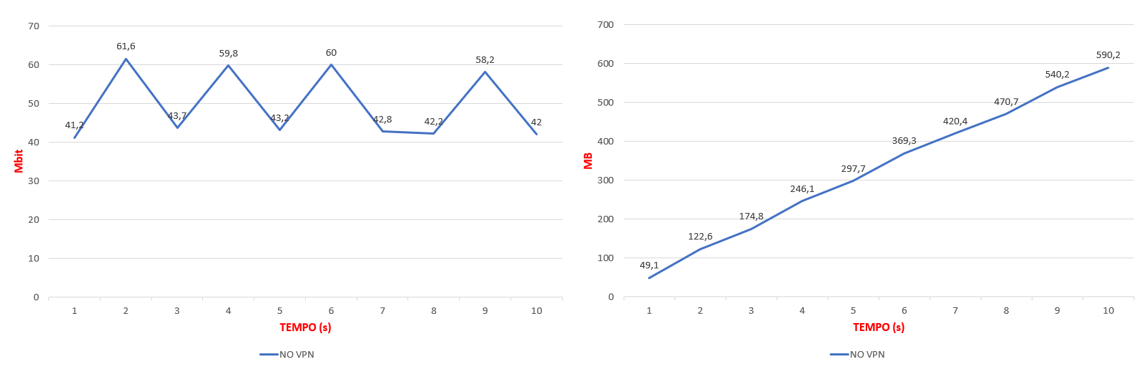
\includegraphics[width=0.9\textwidth] {Tesi magistrale/capitoli/images/16.png}
\centering
\caption{Grafici 10° esecuzione.}
\end{figure}

\newpage
\subsubsection{Grafici esperimento con WireGuard standard}

\begin{figure}[h] 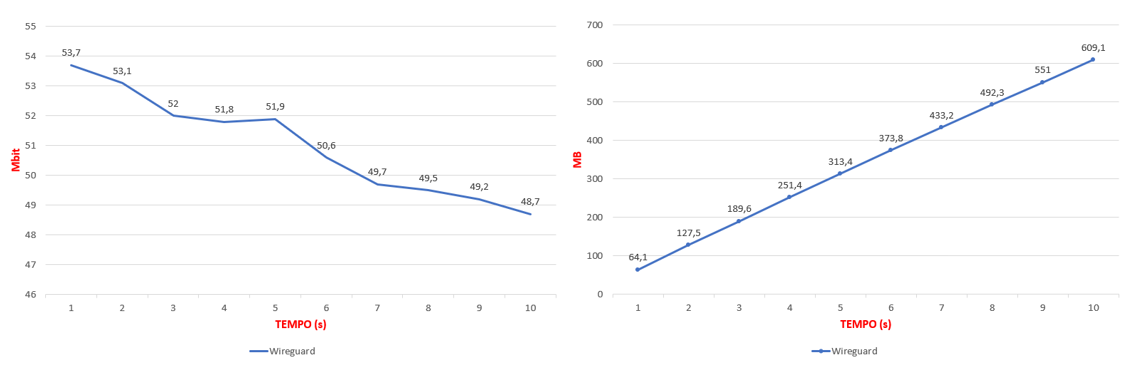
\includegraphics[width=0.9\textwidth] {Tesi magistrale/capitoli/images/17.png}
\centering
\caption{Grafici 1° esecuzione.}
\end{figure}

\begin{figure}[h] 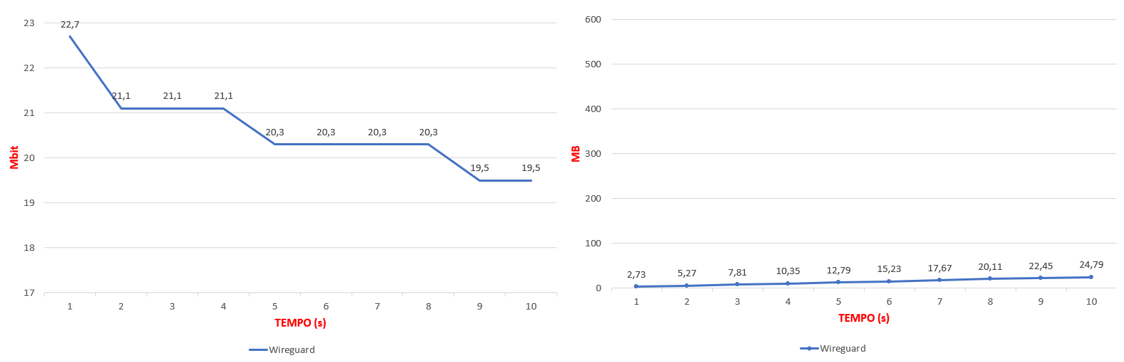
\includegraphics[width=0.9\textwidth] {Tesi magistrale/capitoli/images/18.png}
\centering
\caption{Grafici 5° esecuzione.}
\end{figure}

\begin{figure}[h] 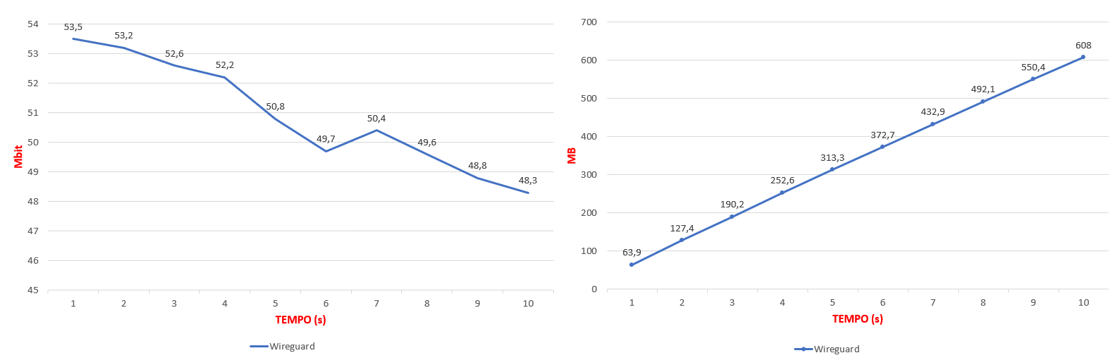
\includegraphics[width=0.9\textwidth] {Tesi magistrale/capitoli/images/19.png}
\centering
\caption{Grafici 10° esecuzione.}
\end{figure}

\newpage
\subsubsection{Grafici esperimento con WireGuard PQ}

\begin{figure}[h] 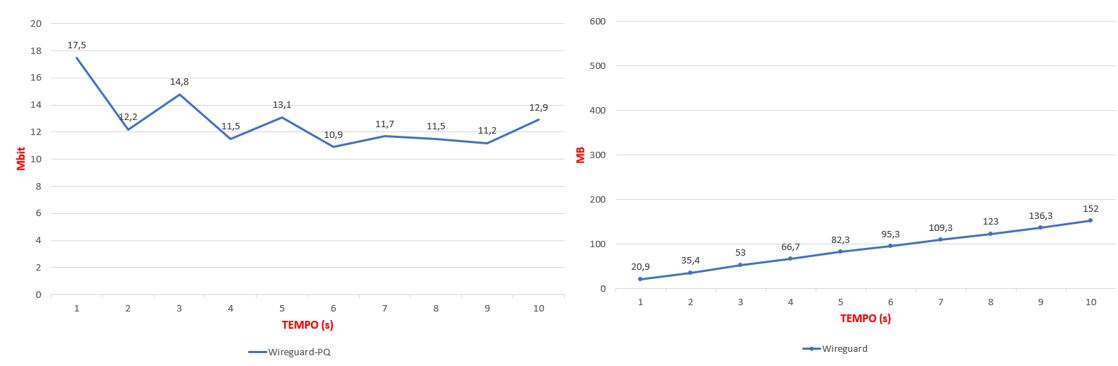
\includegraphics[width=0.9\textwidth] {Tesi magistrale/capitoli/images/20.png}
\centering
\caption{Grafici 1° esecuzione.}
\end{figure}

\begin{figure}[h] 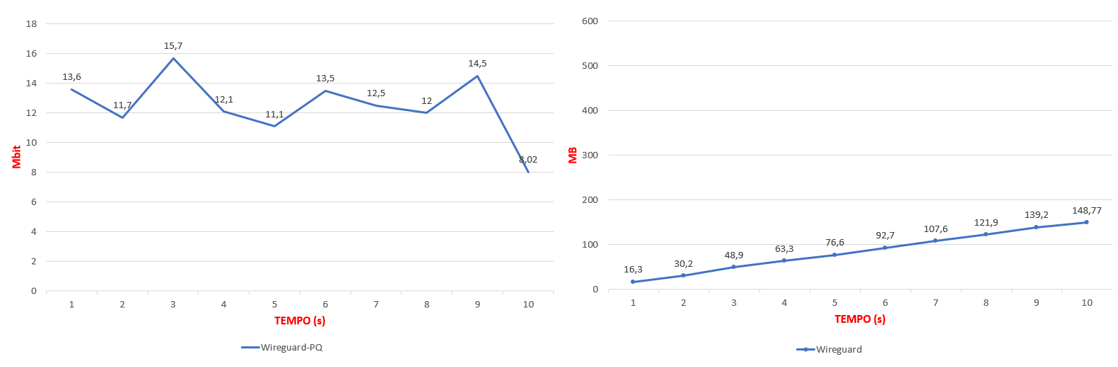
\includegraphics[width=0.9\textwidth] {Tesi magistrale/capitoli/images/21.png}
\centering
\caption{Grafici 5° esecuzione.}
\end{figure}

\begin{figure}[h] 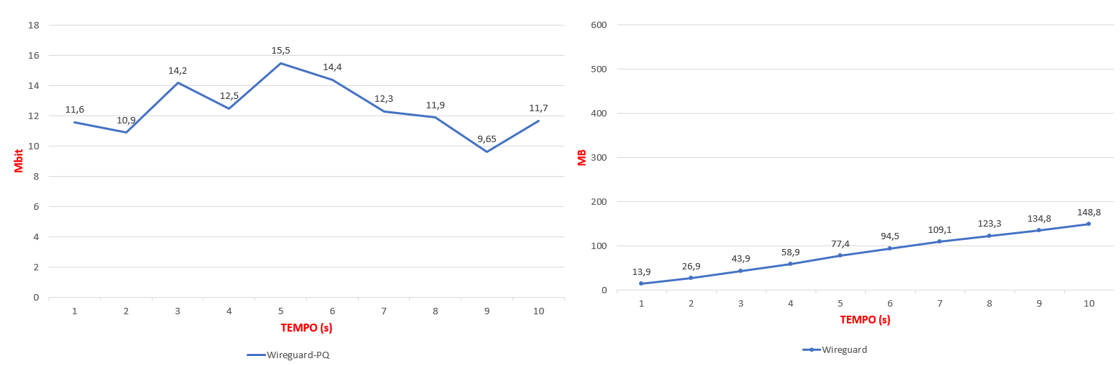
\includegraphics[width=0.9\textwidth] {Tesi magistrale/capitoli/images/22.png}
\centering
\caption{Grafici 10° esecuzione.}
\end{figure}

\newpage
\subsubsection{Grafici esperimento con OpenVPN}

\begin{figure}[h] 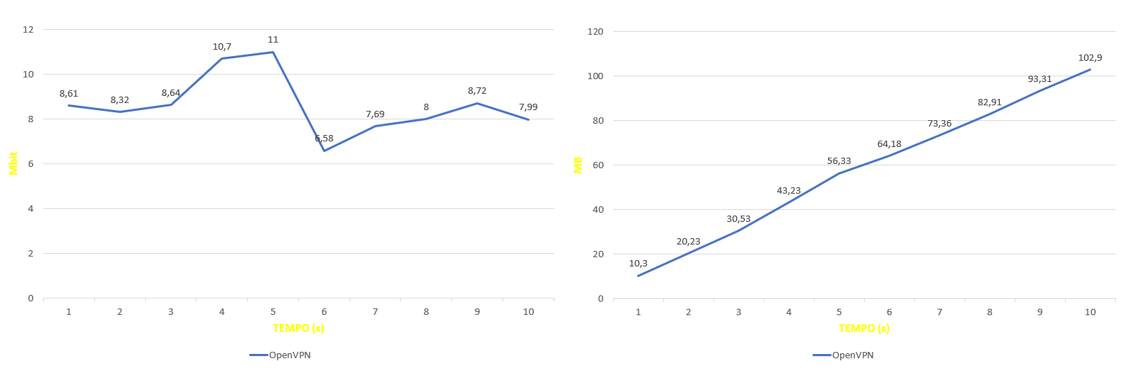
\includegraphics[width=0.9\textwidth] {Tesi magistrale/capitoli/images/23.png}
\centering
\caption{Grafici 1° esecuzione.}
\end{figure}

\begin{figure}[h] 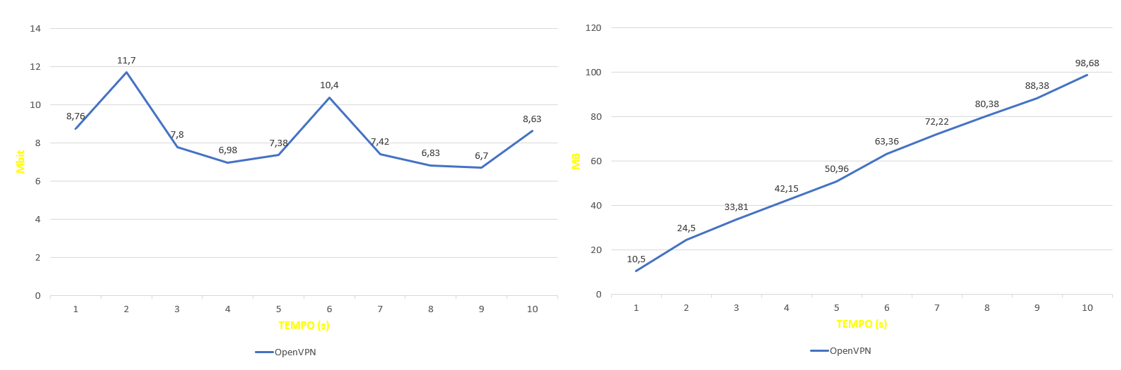
\includegraphics[width=0.9\textwidth] {Tesi magistrale/capitoli/images/24.png}
\centering
\caption{Grafici 5° esecuzione.}
\end{figure}

\begin{figure}[h] 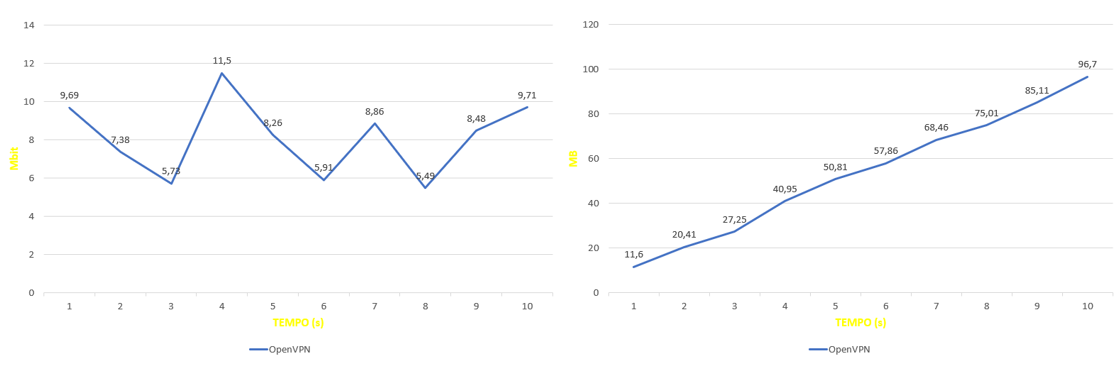
\includegraphics[width=0.9\textwidth] {Tesi magistrale/capitoli/images/25.png}
\centering
\caption{Grafici 10° esecuzione.}
\end{figure}

\newpage
\subsubsection{Grafici riassuntivi}

\begin{figure}[h] 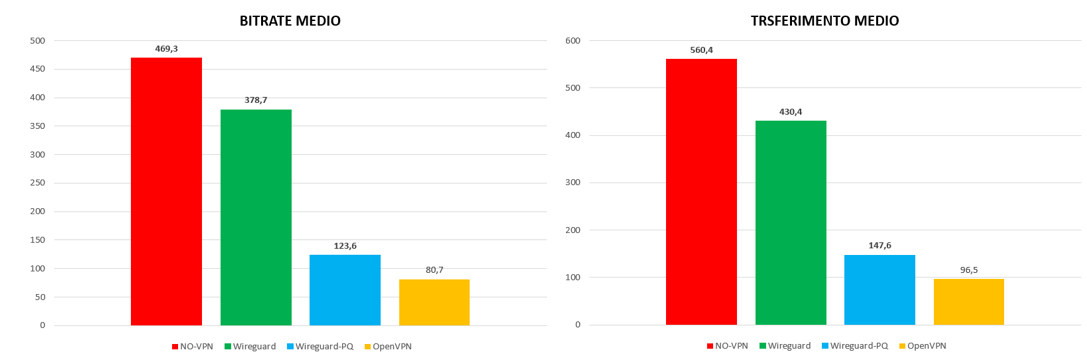
\includegraphics[width=1\textwidth] {Tesi magistrale/capitoli/images/26.png}
\centering
\caption{Grafici riassuntivi.}
\end{figure}

\subsubsection{Esito secondo esperimento}
Come nel primo esperimento, anche in questo caso è ovvio che l'esito sia a favore dell'esecuzione senza impiego di protocolli VPN anche se il divario con essi è abbastanza trascurabile, soprattutto se si considera l'output del test con l'utilizzo di \emph{WireGuard standard}.

\newpage
\subsection{Terzo esperimento}
Questo esperimento riguarda la simulazione di invio di un flusso di dati di livello \emph{applicativo}, in particolare del protocollo \emph{VoIP}.  
\subsubsection{Grafici esperimento senza VPN}

\begin{figure}[h] 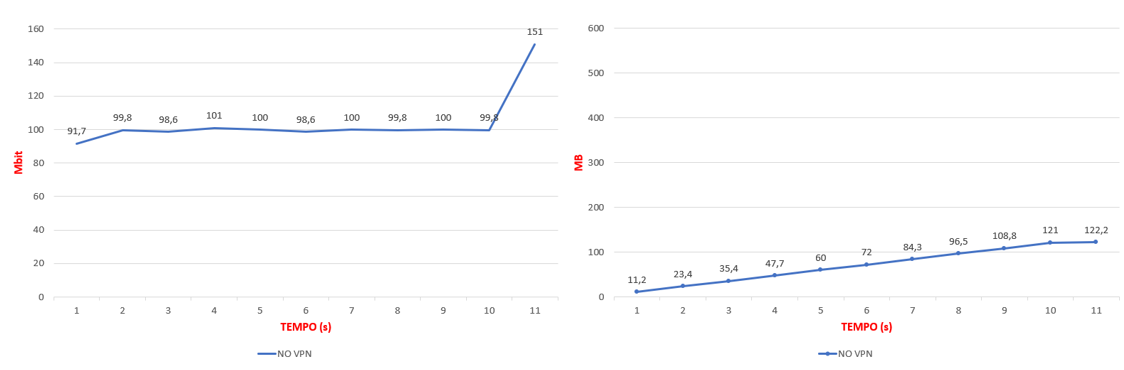
\includegraphics[width=0.9\textwidth] {Tesi magistrale/capitoli/images/27.png}
\centering
\caption{Grafici 1° esecuzione.}
\end{figure}

\begin{figure}[h] 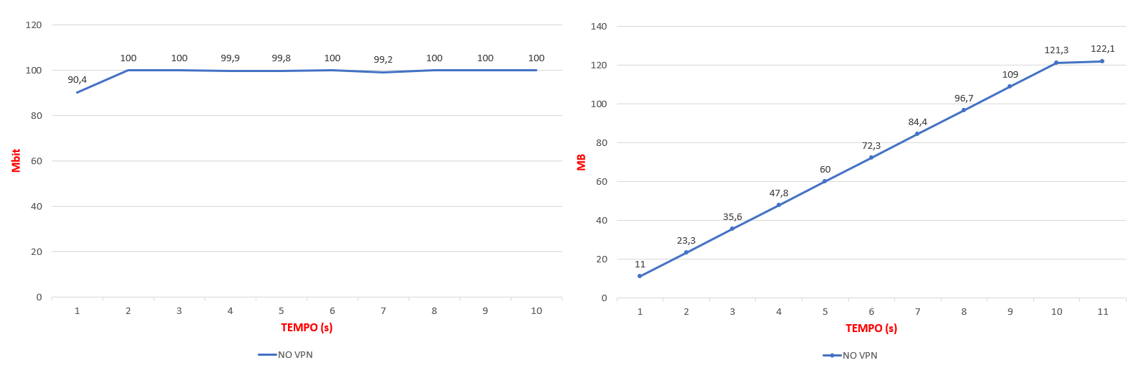
\includegraphics[width=0.9\textwidth] {Tesi magistrale/capitoli/images/28.png}
\centering
\caption{Grafici 5° esecuzione.}
\end{figure}

\begin{figure}[h] 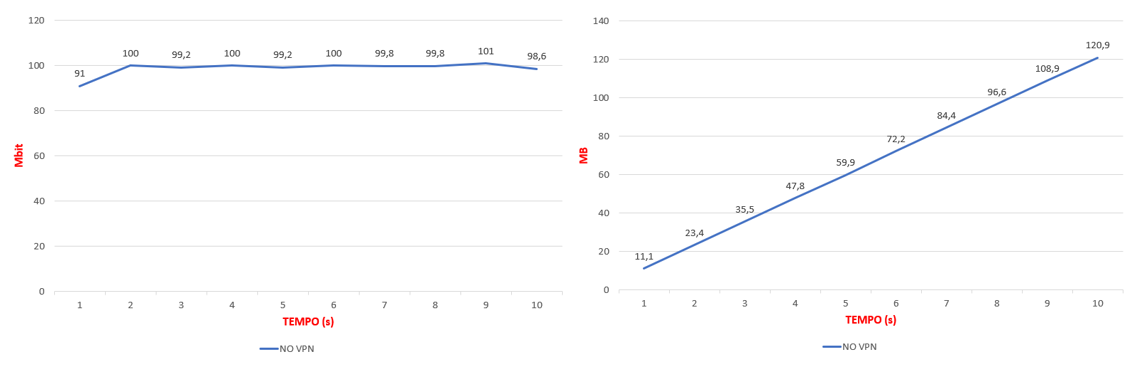
\includegraphics[width=0.9\textwidth] {Tesi magistrale/capitoli/images/29.png}
\centering
\caption{Grafici 10° esecuzione.}
\end{figure}

\newpage
\subsubsection{Grafici esperimento con WireGuard standard}

\begin{figure}[h] 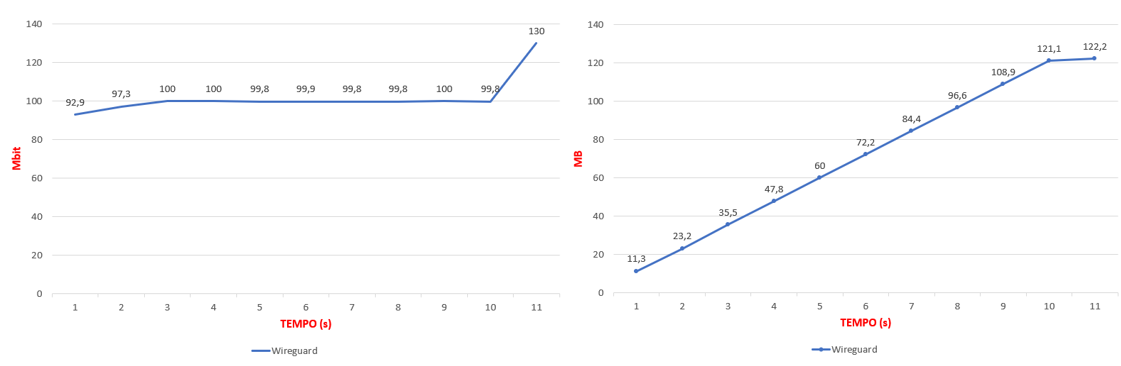
\includegraphics[width=0.9\textwidth] {Tesi magistrale/capitoli/images/30.png}
\centering
\caption{Grafici 1° esecuzione.}
\end{figure}

\begin{figure}[h] 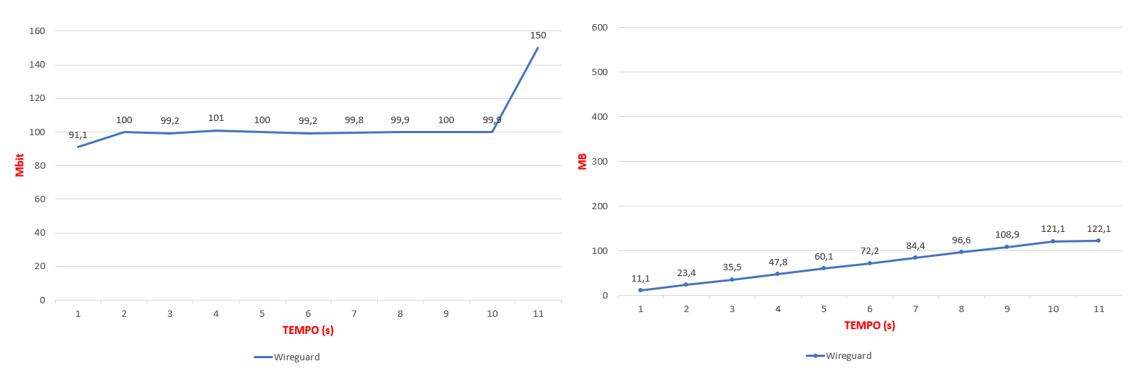
\includegraphics[width=0.9\textwidth] {Tesi magistrale/capitoli/images/31.png}
\centering
\caption{Grafici 5° esecuzione.}
\end{figure}

\begin{figure}[h] 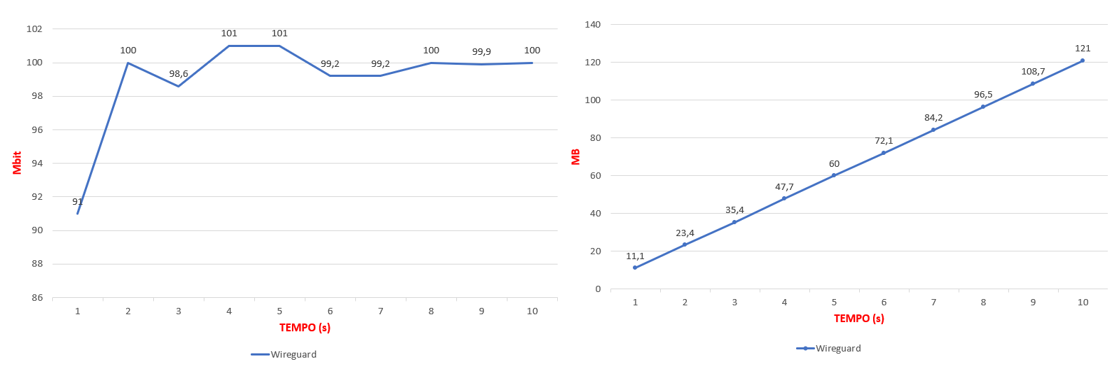
\includegraphics[width=0.9\textwidth] {Tesi magistrale/capitoli/images/32.png}
\centering
\caption{Grafici 10° esecuzione.}
\end{figure}

\newpage
\subsubsection{Grafici esperimento con WireGuard PQ}

\begin{figure}[h] 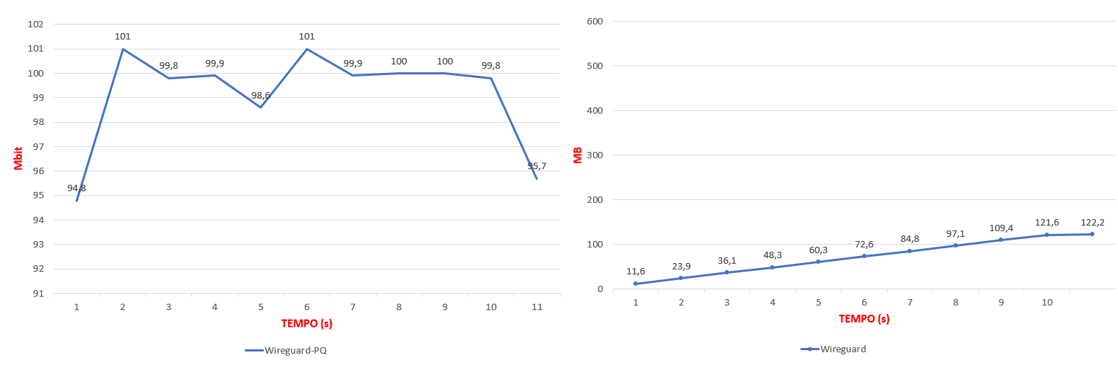
\includegraphics[width=0.9\textwidth] {Tesi magistrale/capitoli/images/33.png}
\centering
\caption{Grafici 1° esecuzione.}
\end{figure}

\begin{figure}[h] 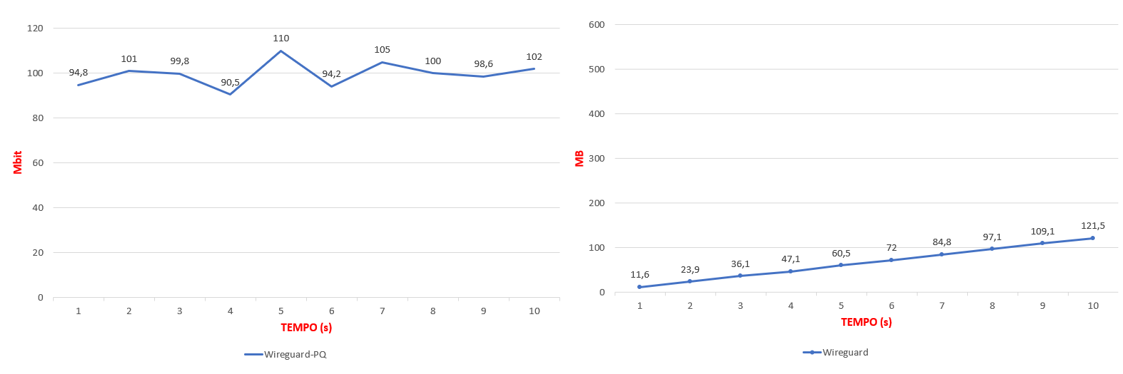
\includegraphics[width=0.9\textwidth] {Tesi magistrale/capitoli/images/34.png}
\centering
\caption{Grafici 5° esecuzione.}
\end{figure}

\begin{figure}[h] 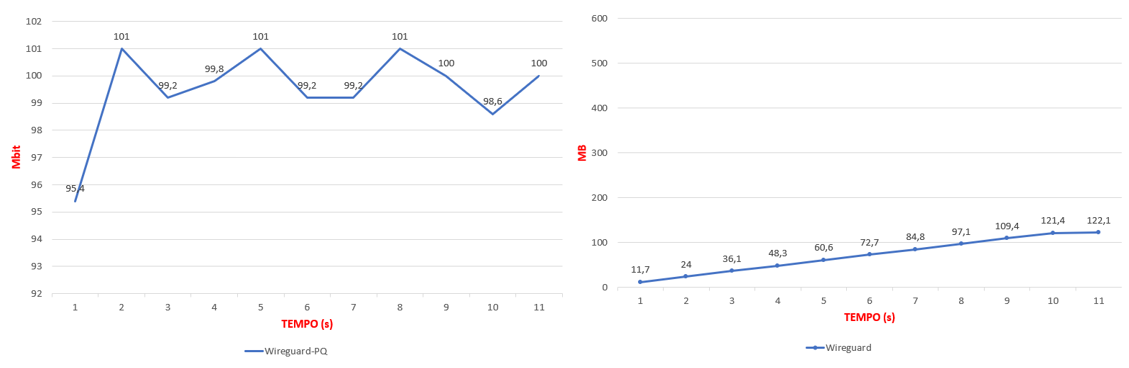
\includegraphics[width=0.9\textwidth] {Tesi magistrale/capitoli/images/35.png}
\centering
\caption{Grafici 10° esecuzione.}
\end{figure}

\newpage
\subsubsection{Grafici esperimento con OpenVPN}

\begin{figure}[h] 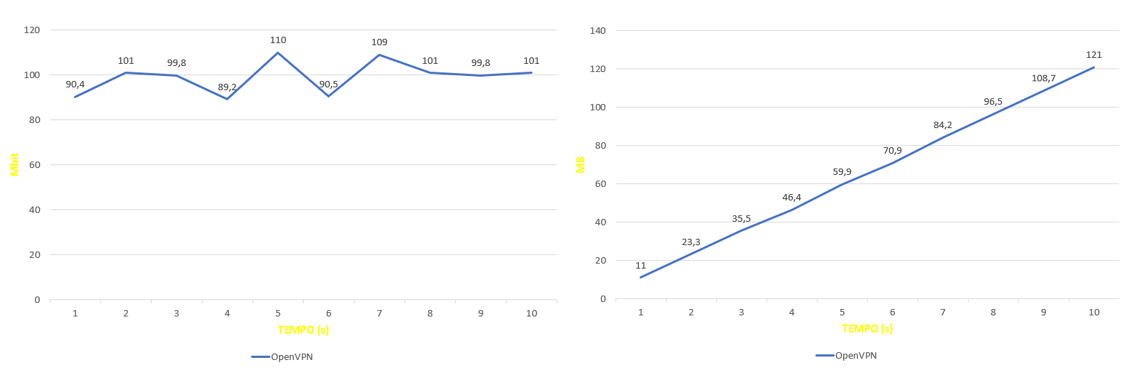
\includegraphics[width=0.9\textwidth] {Tesi magistrale/capitoli/images/42.png}
\centering
\caption{Grafici 1° esecuzione.}
\end{figure}

\begin{figure}[h] 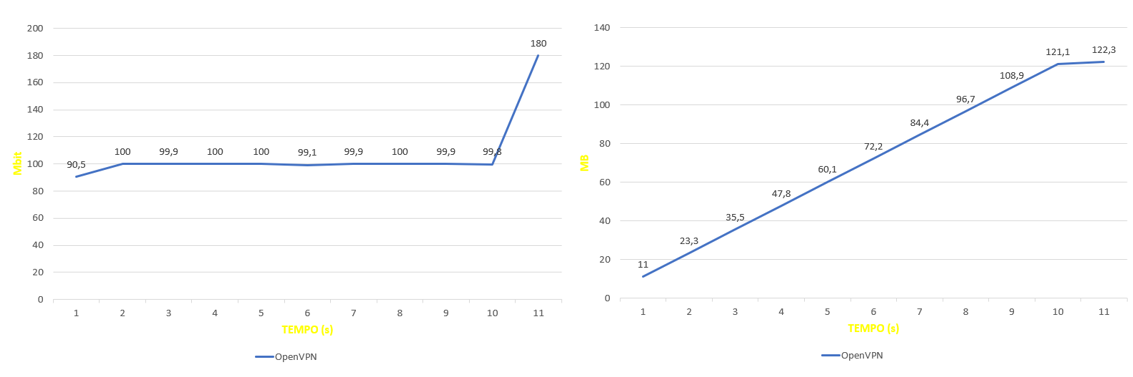
\includegraphics[width=0.9\textwidth] {Tesi magistrale/capitoli/images/43.png}
\centering
\caption{Grafici 5° esecuzione.}
\end{figure}

\begin{figure}[h] 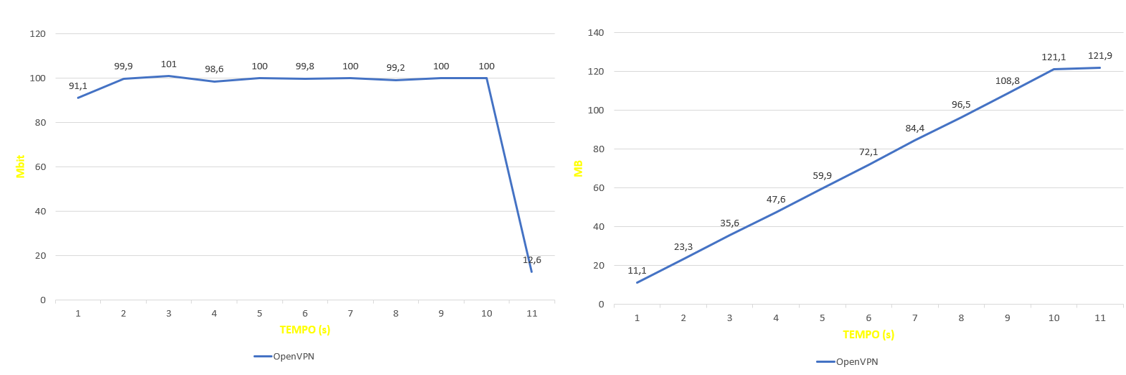
\includegraphics[width=0.9\textwidth] {Tesi magistrale/capitoli/images/44.png}
\centering
\caption{Grafici 10° esecuzione.}
\end{figure}

\newpage
\subsubsection{Grafici riassuntivi}

\begin{figure}[h] 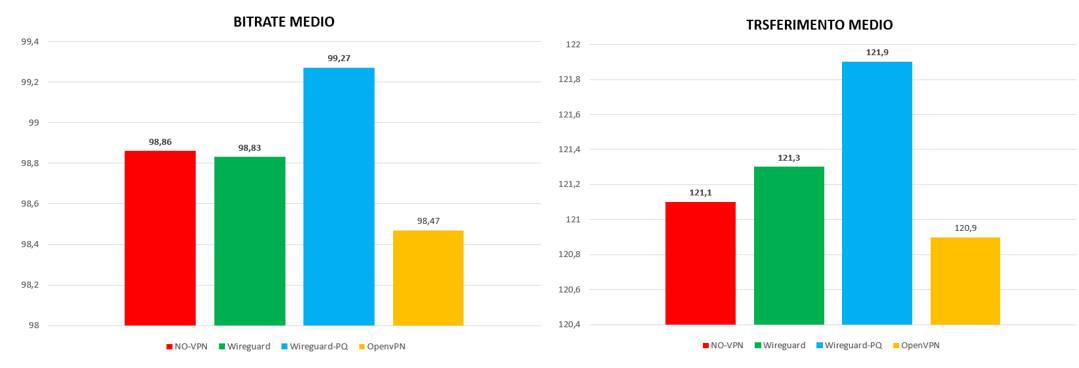
\includegraphics[width=1\textwidth] {Tesi magistrale/capitoli/images/36.png}
\centering
\caption{Grafici riassuntivi.}
\end{figure}

\subsubsection{Esito terzo esperimento}
Sorprendenmente nonostante il protocollo \emph{WireGuard PQ} sia oggettivamente più complesso data la sua natura, riesce, se pur leggermente, a sovrastare gli altri protocolli VPN testati e a superare addirittura l'esito del test senza l'utilizzo di VPN. 

\newpage
\subsection{Quarto esperimento}
Questo esperimento è stato ideato con l'obiettivo di simulare l'invio di pacchetti TCP appartenenti ad un flusso di dati adibito allo streaming video, come ad esempio \emph{Netflix}
\subsubsection{Grafici esperimento senza VPN}

\begin{figure}[h] \includegraphics[width=0.9\textwidth] {Tesi magistrale/capitoli/images/37.png}
\centering
\caption{Grafici 1° esecuzione.}
\end{figure}

\begin{figure}[h] \includegraphics[width=0.9\textwidth] {Tesi magistrale/capitoli/images/38.png}
\centering
\caption{Grafici 5° esecuzione.}
\end{figure}

\begin{figure}[h] \includegraphics[width=0.9\textwidth] {Tesi magistrale/capitoli/images/39.png}
\centering
\caption{Grafici 10° esecuzione.}
\end{figure}

\newpage
\subsubsection{Grafici esperimento con WireGuard standard}

\begin{figure}[h] \includegraphics[width=0.9\textwidth] {Tesi magistrale/capitoli/images/40.png}
\centering
\caption{Grafici 1° esecuzione.}
\end{figure}

\begin{figure}[h] \includegraphics[width=0.9\textwidth] {Tesi magistrale/capitoli/images/41.png}
\centering
\caption{Grafici 5° esecuzione.}
\end{figure}

\begin{figure}[h] \includegraphics[width=0.9\textwidth] {Tesi magistrale/capitoli/images/45.png}
\centering
\caption{Grafici 10° esecuzione.}
\end{figure}

\newpage
\subsubsection{Grafici esperimento con WireGuard PQ}

\begin{figure}[h] \includegraphics[width=0.9\textwidth] {Tesi magistrale/capitoli/images/46.png}
\centering
\caption{Grafici 1° esecuzione.}
\end{figure}

\begin{figure}[h] \includegraphics[width=0.9\textwidth] {Tesi magistrale/capitoli/images/47.png}
\centering
\caption{Grafici 5° esecuzione.}
\end{figure}

\begin{figure}[h] \includegraphics[width=0.9\textwidth] {Tesi magistrale/capitoli/images/48.png}
\centering
\caption{Grafici 10° esecuzione.}
\end{figure}

\newpage
\subsubsection{Grafici esperimento con OpenVPN}

\begin{figure}[h] \includegraphics[width=0.9\textwidth] {Tesi magistrale/capitoli/images/49.png}
\centering
\caption{Grafici 1° esecuzione.}
\end{figure}

\begin{figure}[h] \includegraphics[width=0.9\textwidth] {Tesi magistrale/capitoli/images/50.png}
\centering
\caption{Grafici 5° esecuzione.}
\end{figure}

\begin{figure}[h] \includegraphics[width=0.9\textwidth] {Tesi magistrale/capitoli/images/51.png}
\centering
\caption{Grafici 10° esecuzione.}
\end{figure}

\newpage
\subsubsection{Grafici riassuntivi}

\begin{figure}[h] \includegraphics[width=1\textwidth] {Tesi magistrale/capitoli/images/52.png}
\centering
\caption{Grafici riassuntivi.}
\end{figure}

\subsubsection{Esito quarto esperimento}
Per quanto riguarda questo esperimento, il comportamento migliore è stato ottenuto senza l'impiego di protocolli VPN mentre con essi sono stati ottenuti dei risultati che dimostrano chiaramente che la differenza prestazionale è abbastanza ampia, soprattutto se si considerano i protocolli \emph{WireGuard PQ} e \emph{OpenVPN}.

\newpage
\subsection{Quinto esperimento}
l'ultimo esperimento eseguito riguarda il trasferimento massivo di dati, in particolare i pacchetti appartengono ad un flusso di trasferimento massivo di tipo TCP.

\subsubsection{Grafici esperimento senza VPN}

\begin{figure}[h] \includegraphics[width=0.9\textwidth] {Tesi magistrale/capitoli/images/53.png}
\centering
\caption{Grafici 1° esecuzione.}
\end{figure}

\begin{figure}[h] \includegraphics[width=0.9\textwidth] {Tesi magistrale/capitoli/images/54.png}
\centering
\caption{Grafici 5° esecuzione.}
\end{figure}

\begin{figure}[h] \includegraphics[width=0.9\textwidth] {Tesi magistrale/capitoli/images/55.png}
\centering
\caption{Grafici 10° esecuzione.}
\end{figure}

\newpage
\subsubsection{Grafici esperimento con WireGuard standard}

\begin{figure}[h] \includegraphics[width=0.9\textwidth] {Tesi magistrale/capitoli/images/56.png}
\centering
\caption{Grafici 1° esecuzione.}
\end{figure}

\begin{figure}[h] \includegraphics[width=0.9\textwidth] {Tesi magistrale/capitoli/images/57.png}
\centering
\caption{Grafici 5° esecuzione.}
\end{figure}

\begin{figure}[h] \includegraphics[width=0.9\textwidth] {Tesi magistrale/capitoli/images/58.png}
\centering
\caption{Grafici 10° esecuzione.}
\end{figure}

\newpage
\subsubsection{Grafici esperimento con WireGuard PQ}

\begin{figure}[h] \includegraphics[width=0.9\textwidth] {Tesi magistrale/capitoli/images/59.png}
\centering
\caption{Grafici 1° esecuzione.}
\end{figure}

\begin{figure}[h] \includegraphics[width=0.9\textwidth] {Tesi magistrale/capitoli/images/60.png}
\centering
\caption{Grafici 5° esecuzione.}
\end{figure}

\begin{figure}[h] \includegraphics[width=0.9\textwidth] {Tesi magistrale/capitoli/images/61.png}
\centering
\caption{Grafici 10° esecuzione.}
\end{figure}

\newpage
\subsubsection{Grafici esperimento con OpenVPN}

\begin{figure}[h] \includegraphics[width=0.9\textwidth] {Tesi magistrale/capitoli/images/62.png}
\centering
\caption{Grafici 1° esecuzione.}
\end{figure}

\begin{figure}[h] \includegraphics[width=0.9\textwidth] {Tesi magistrale/capitoli/images/63.png}
\centering
\caption{Grafici 5° esecuzione.}
\end{figure}

\begin{figure}[h] \includegraphics[width=0.9\textwidth] {Tesi magistrale/capitoli/images/64.png}
\centering
\caption{Grafici 10° esecuzione.}
\end{figure}

\newpage
\subsubsection{Grafici riassuntivi}

\begin{figure}[h] \includegraphics[width=1\textwidth] {Tesi magistrale/capitoli/images/65.png}
\centering
\caption{Grafici riassuntivi.}
\end{figure}

\subsubsection{Esito quinto esperimento}
Anche in questo caso, come per diversi altri esperimenti, è evidente che l'utilizzo di protocolli VPN possa influenzare 
notevolmente le prestazioni di rete disponibili, spesso causando un decremento notevole come ad esempio nel caso del test eseguito con il protocollo \emph{OpenVPN}.
\chapter{Conclusioni e sviluppi Futuri} %\label{1cap:spinta_laterale}
% [titolo ridotto se non ci dovesse stare] {titolo completo}
%


\begin{citazione}
In questa sezione, saranno riassunti i risultati ottenuti dal sistema realizzato, ed inoltre, saranno discussi i potenziali sviluppi che potrebbero essere intrapresi in futuro.
\end{citazione}
\newpage

\section{Risultati ottenuti}
Una volta che il sistema è stato implementato correttamente, tutti i test sono stati portati avanti come spiegato nel capitolo precedente in modo da poter stabilire con sicurezza il \emph{comportamento} di ognuno dei protocolli VPN impiegati affinché sia chiaro quale sia quello più adatto da utilizzare in relazione anche al grado di \emph{sicurezza} che si vuole ottenere. Come si è potuto osservare dai risultati prodotti dalle esecuzioni degli esperimenti, ognuno di essi ha dato un output diverso condizionato principalmente dal fatto che alla base di ogni tentativo eseguito è presente un flusso di dati differente per ognuno di essi.

\subsection{Valutazione dei risultati}
Osservando i grafici e quindi gli output relativi alle esecuzioni degli esperimenti, si può facilmente notare che per ognuno di essi il risultato è distinto, in particolare:
\begin{itemize}
    \item \emph{Esperimento 1}: WireGuard standard è il protocollo VPN a comportarsi meglio;
    \item \emph{Esperimento 2}: WireGuard standard è il protocollo VPN a comportarsi meglio;
    \item \emph{Esperimento 3}: WireGuard PQ è il protocollo VPN a comportarsi meglio;
    \item \emph{Esperimento 4}: WireGuard standard è il protocollo VPN a comportarsi meglio;
    \item \emph{Esperimento 5}: Wireguard standard è il protocollo VPN a comportarsi meglio.
\end{itemize}

Dall'elenco superiore si intuisce che in linea di massima il protocollo \emph{WireGuard} si comporta meglio del protocollo \emph{OpenVPN} con questi precisi esperimenti eseguiti; in particolare la versione \emph{standard} risulta offrire le migliori prestazioni mentre la versione \emph{PQ} ha restituito in output dei risultati che sono perfettamente paragonabili a quelli ottenuti utilizzando OpenVPN, il quale conferma che nonostante l'\emph{overhead} aggiunto a causa degli algoritmi \emph{Post Quantum} impiegati da WireGuard PQ esso risulta comunque prestazionalmente paragonabile ad un protocollo VPN che impiega algoritmi convenzionali. 

\section{Contributi della ricerca}
Arrivati a questo punto del percorso affrontato, è importante notare qual'è il \emph{contributo} effettivo che il presente progetto può offrire alla ricerca ed allo sviluppo di soluzioni post quantum inerenti al trasferimento di flussi di dati aventi determinate esigenze in termini di rete. Il lavoro portato avanti ha consentito di realizzare uno strumento che al giorno d'oggi può essere di grande aiuto soprattutto per quei settori della ricerca che sono strettamente correlati allo sviluppo di nuovi algoritmi post quantum ed al trasferimento sicuro di dati. La testbed realizzata offre la possibilità di poter eseguire numerosi test e di poter integrare anche altri algoritmi in modo da poter effettuare una comparazione dei protocolli VPN ancora più ampia ed esaustiva. Inerentemente ai flussi di dati trasferiti, il tool \emph{Iperf} ha consentito di poter simulare in modo preciso e rapido l'insieme di flussi impiegati durante gli esperimenti, ma offre la possibilità di poterne simulare tanti altri così da approfondire le performance e/o testare altri parametri di rete come il \emph{packet loss}.
\section{Sviluppi futuri}
Analizziamo ora alcune delle possibili strade che potrebbero essere intraprese al fine di apportare delle migliorie al lavoro svolto, sia per quanto riguarda le funzionalità realizzate che lo studio portato avanti.

\subsection{Ulteriori esperimenti}
Come accennato nel paragrafo precedente, in futuro potrebbe essere sicuramente utile progettare ed eseguire diversi altri esperimenti i quali fanno riferimento a differenti flussi di dati aventi requisiti diversi da quelli previsti in questo lavoro. Questo tipo di sviluppo potrebbe fare ulteriore chiarezza sui protocolli VPN in modo da stabilire con certezza quali di essi sono più adatti a determinati scopi.

\subsection{Infrastruttura di rete}
In relazione alle performance ottenute dai protocolli VPN testati tramite gli esperimenti eseguiti, potrebbe essere interessante ripetere questi ultimi fornendo alla testbed delle \emph{connessioni di rete} diverse da quella impiegata in questo lavoro così da poter analizzare i risultati anche in relazione al tipo di connessione che si sta utilizzando per connettere la testbed in rete.

\subsection{Realizzazione interfaccia web}
Le funzionalità proposte agli utenti che intendono farne uso, in particolare il modulo inerente all'esecuzione delle scansioni di rete tramite l'uso della libreria \emph{Nmap}, sono state pensate per essere sfruttate tramite delle \emph{richieste HTTP} eseguite dagli host presenti in rete LAN; a tale proposito sarebbe efficace sviluppare una \emph{GUI} il quale semplificherebbe di gran lunga l'esecuzione delle richieste, soprattutto ad un pubblico che non ha molta dimestichezza con la generazione delle richieste manualmente o banalmente per avvantaggiare la fruizione delle funzionalità stesse.




\backmatter
\phantomsection
\chapter{Ringraziamenti}
\markboth{Ringraziamenti}{}
% [titolo ridotto se non ci dovesse stare] {titolo completo}

Con la realizzazione di quest'ultimo lavoro termina la mia carriera accademica il quale oltre ad avermi permesso di approfondire la mia principale passione e di poterne farne un lavoro, in futuro, mi ha fatto capire fino in fondo cosa significhi avere vicino le giuste persone ed il conseguente impatto che influisce a lungo termine sulla vita quotidiana. il percorso accademico affrontato è stato avvolto da un contesto non proprio ideale ad esso ed è per tale motivo che intendo ringraziare le giuste persone che hanno contribuito positivamente a migliorarlo.

Ringrazio innanzitutto il \emph{Prof. Arcangelo Castiglione}; ha sempre riposto le giuste attenzioni allo sviluppo del lavoro proposto e alla risoluzione immediata dei problemi riscontarti lungo il percorso. Nutro nei suoi confronti un grande senso di stima in particolare per la dedizione che ripone nel suo lavoro.

Ringrazio \emph{Marco}; oltre a fornire costante supporto sia al progetto che morale, hai creduto sin dall'inizio in me dandomi la possibilità di poter collaborare con te e gli altri colleghi di \emph{BSQ Security}. Grazie a te ho potuto apprendere nuove conoscenze ed un ottimo approccio al mondo lavoro.

Ringrazio \emph{Lorenzo}; ti sei rivelato un sincero amico oltre che affidabile compagno di tanti avvenimenti; ho sempre potuto contare su di te nei momenti in cui avevo bisogno e per questo ti sono riconoscente. Spero che quest'amicizia possa continuare ancora per molto tempo nonostante gli inconvenienti che incontreremo sulle nostre strade.

Ringrazio \emph{Vincenzo}; con te ho trascorso gran parte dell'ultimo anno accademico durante il quale ho imparato a conoscerti meglio; con il tempo ho capito che siamo molto più simili di quanto avremmo mai potuto dire qualche anno fa e questo mi ha dato la possibilità di confrontarmi spesso con te su diversi argomenti. Ti ringrazio per le lunghe chiacchierate e per avermi sempre ascoltato seriamente. 

Ringrazio \emph{Carmen}; per avermi offerto da sempre il tuo supporto soprattutto nelle situazioni più spinose, grazie a te ho trovato una vera amica capace di dare il giusto sostegno in qualsiasi circostanza e di ascoltare sempre in maniera garbata, talvolta strappando anche una risata. 

Ringrazio \emph{Simone}; nonostante quest'ultimo periodo sia stato abbastanza movimentato per entrambi hai da sempre trovato il modo di offrire la giusta attenzione al nostro rapporto e di esserci attivamente per qualsiasi situazione. Confido nel fatto che la nostra amicizia possa proseguire ancora per molto tempo.

Ringrazio i miei \emph{parenti}; per avermi sempre sostenuto senza intralciare le mie scelte ed al contempo dare il sostegno necessario per intraprenderle. Siete stati di fondamentale importanza per il raggiungimento di un obiettivo così importante per me.

Ringrazio \emph{Carmen P.}; sei e sarai il mio punto di riferimento sulla quale posso fare costantemente affidamento in qualsiasi situazione. A te va il mio più sincero ringraziamento.

Infine, ringrazio tutti i miei \emph{amici} e quelle persone che hanno avuto la premura di compiere anche una singola azione positiva nei miei confronti, spronandomi a continuare il mio percorso. 

Vi sarò per sempre riconoscente.
%*******************************************************
% Bibliografia
%*******************************************************
\cleardoublepage
\phantomsection
\addcontentsline{toc}{chapter}{\bibname}
\nocite{*}
\bibliographystyle{unsrt}
{ \setstretch{1.3}
\bibliography{bibliografia}
}
\vspace{0.5cm}
% \begin{Large}Fonti\end{Large}
% \begin{itemize}
% \end{itemize}


\end{document}
